\documentclass[acmsmall,timestamp,review]{acmart}

% Packages {{{
\usepackage{hyperref}
\usepackage{amsmath}
\usepackage{amssymb}
\usepackage{bbm}
\usepackage{tikz}
\usetikzlibrary{calc}
\usetikzlibrary{graphs}
\usetikzlibrary{cd}
\usepackage{bussproofs}
\usepackage{stmaryrd}
\usepackage{calc}
\usepackage{bbm}
% }}}

% Parameters {{{

\hyphenation{Comp-Cert}

% }}}

% Macros {{{

%\newtheorem{example}{Example}
%\newtheorem{definition}{Definition}
%\newtheorem{lemma}{Lemma}

\newcommand{\kw}[1]{\ensuremath{ \mathsf{#1} }}
\newcommand{\ifr}[1]{\ [{#1}]\ }
\newcommand{\ifrw}[2]{\ [{#1}]_{#2}\ }
\newcommand{\alt}{\ |\ } % use \mid instead
\newcommand{\bind}{\gg\!\!=}

\newcommand{\EC}{\kw{C}}
\newcommand{\simrel}{\kw{simrel}}

% Moves
\newcommand{\mcall}[3]{\kw{#1}({#2})@{#3}}
\newcommand{\pcall}[3]{%
  \underline{\mcall{#1}{#2}{#3}}%
}
\newcommand{\mret}[2]{{#1}@{#2}}
\newcommand{\pret}[2]{%
  \underline{\mret{#1}{#2}}%
}
\newcommand{\mretx}[3]{{#1}@{#2}/{#3}}
\newcommand{\pretx}[3]{%
  \underline{\mretx{#1}{#2}{#3}}%
}

% Pointers for justified sequences %{{{

% Parameters
\newcommand{\pshift}{1.6ex}
\newcommand{\pcdist}{2.5}
\newcommand{\pcangle}{60}

% Pointer hook
\newcommand{\ph}[1]{%
  \tikz[remember picture]{\coordinate (#1);}}

% Pointer to
\newcommand{\pt}[1]{%
  \rule{0pt}{1.4em}%
  \tikz[remember picture, overlay]{
    \draw[->]
      let \p{dest} = (#1),
          \n1 = {ln(veclen(\x{dest}, \y{dest}) + 1)},
          \p1 = ($(0,0)+(0,\pshift)$),
          \p4 = ($(#1)+(0,\pshift)$),
          \p2 = ($(\p1)!\n1*\pcdist!-\pcangle:(\p4)$),
          \p3 = ($(\p4)!\n1*\pcdist!+\pcangle:(\p1)$) in
        (\p1) .. controls (\p2) and (\p3) .. (\p4);}}

%}}}

% }}}

\title{Refinement-Based Game Semantics as
  a Calculus for Certified Components}

\author{J\'er\'emie Koenig}
\affiliation{Yale University}
\email{jeremie.koenig@yale.edu}

\author{Zhong Shao}
\affiliation{Yale University}
\email{zhong.shao@yale.edu}

\begin{document}

\begin{abstract} %{{{
In recent years,
formal verification of computer systems
of increasing size has become practical.
Researchers have been able to verify complex artifacts
at a variety of abstraction levels spanning
from CPU designs to network protocols.

These achievements remain discrete efforts, but
there has been increasing interest in rendering them interoperable,
as exemplified by the DeepSpec project.
The ability to connect correctness proofs of components
verified at various levels of abstraction
would enable the construction of extremely reliable heterogenous systems
through end-to-end verification.

In this paper,
we propose that a successful synthesis of existing research on
game semantics,
refinement-based methods,
abstraction layers and
logical relations
has the potential to serve as a common theory
of certified components.
\end{abstract}
%}}}

\maketitle

\section{Introduction} %{{{

% preamble {{{

Recent years have seen rapid progress in the field of formal methods.
In particular,
researchers have been able to formally verify the
total functional correctness
of various key components of computer systems
of significant complexity,
including
compilers \cite{compcert, vellvm},
operating system kernels \cite{sel4, popl15},
file systems \cite{fscq}, and
processor designs \cite{safe}.
Such verification efforts
consist of
a formal semantics describing the system's behavior,
a formal specification of the system's requirements and
the guarantees we wish to establish,
and a mechanized proof that
the system indeed conforms to the specification.
Assuming the semantic model and specification accurately describe
the system's operation and requirements,
this approach can provide
extremely strong reliability and security guarantees.
Moreover,
if the proof is mechanized in a general-purpose proof assistant,
it can be validated by a third-party with minimal effort
and without the need to trust the original developers.

%}}}

\subsection{Specifications as Intefaces} %{{{

Such achievements remain discrete efforts, but
there has been increasing interest in rendering them interoperable,
as exemplified by the DeepSpec project \cite{deepspec}.
By using formal specifications as interfaces
between the correctness proofs of various components ---
showing that the requirements of one component
are met by the guarantees of another ---
the researchers in DeepSpec hope to
obtain formal guarantees about composite systems
operating over a wide range of abstraction layers.
If successful,
such an achievement would represent a deployment of formal methods
at a scale far beyond the current state of the art.

In addition,
this approach could provide reliability and security guarantees
even beyond those of existing formally verified components.
A certified component is only as trustworthy as its specification;
having specifications tied too much to a single verification effort
increases the risk of
implementation bugs being simply propagated to
the specification.
These bugs would become apparent in an effort to
connect the specification's guarantees to
the requirements of another component.
In addition,
specifications used as internal interfaces
in a larger certified system cease to be part of
the overall system's trusted base;
in this way,
building larger certified systems
by composing existing ones
would reduce the
ratio between the size of the external specification to
the overall size of the system.

%}}}

\subsection{Challenges} %{{{

At present, many verification projects
use ad-hoc semantic models and specifications,
expressed in paradigms chosen first and foremost
to render modeling and verification tasks tractable.
Since verification is challenging,
the freedom to choose an appropriate semantic model
is quite desirable.
On the other hand,
the diversity of paradigms used for specification and verification
makes it difficult
to interface projects using different approaches.
These competing concerns
suggest the need to identify a common,
flexible semantic framework
into which existing models could be embedded
for integration purposes.

To enable the construction of certified systems
by assembling off-the-shelf components,
this framework should be equipped with
a rich composition infrastructure
and high-level principles for
reasoning about composite systems.
This represent another point of tension
between the operational models
often used for verification,
and denotational models
that feature compositionality and
support equational reasoning.

%}}}

\subsection{Contributions} %{{{

In this paper,
we argue that
a successful synthesis of existing research
on game semantics,
refinement-based verification,
and certified abstraction layers
could provide a general framework
for the construction of large-scale certified systems.
We call this approach \emph{refinement-based game semantics}.

In \S\ref{sec:mainideas},
we examine from a more formal perspective
the principles enabling the construction
of large-scale certified systems.
We describe our high-level vision of
refinement-based game semantics,
and explain the ways in which
[we think it's up to the task].

Our first technical contribution
appears in \S\ref{sec:monad}:
we construct a semantic framework, formalized in the Coq proof assistant,
by enriching a simple game model
with abstraction and refinement,
and show how a traditional
trace-based strategy model
can be made more amenable to operational reasoning
by enriching it with monadic structure.

While our game model remains much simpler than
those used in the semantics of high-order
functional programming languages,
we demonstrate its applicability in \S\ref{sec:modsem}
by using it to formulate a compositional module semantics
for CompCert.
In contrast with previous attempts \cite{compcompcert,cpp15},
our model incorporates a full account of abstraction,
taking into account the differences in
the nature of cross-module communication
between the different languages involved in CompCert.

This is used to full effect in \S\ref{sec:compcert},
where we show that a high-level
\emph{calling convention algebra}
can be used to render the correctness theorem of CompCert
fully compositional,
with only minimal changes to the existing correctness proofs
of compiler passes.

%}}}

%}}}

\section{Main Ideas} \label{sec:mainideas} %{{{

\subsection{Principles for system construction} %{{{

% preamble {{{

The goal of certified system design is
to create a formal description of
the system to be constructed (the program),
while ensuring through careful analysis that the system
will behave properly.

To carry out this analysis,
we need to assign
to each possible system description $p \in P$
a mathematical object $\llbracket p \rrbracket \in \mathbb{D}$
representing its behavior.
We will call the set $\mathbb{D}$ a \emph{semantic domain}.
In this section we elucidate
the structure and properties of $\mathbb{D}$
necessary to the process of builing
large-scale certified systems.

%}}}

\subsubsection{Specifications and refinement} %{{{

System design starts with a set of requirements
that constrain the behavior of the system to be constructed
(the specification).
These requirements may not capture every detail
of the behavior of the eventual system,
but instead delineate the range of acceptable behaviors
from the point of view of its environment.

In refinement-based approaches,
programs and specifications are interpreted in the same
semantic domain $\mathbb{D}$,
which is equipped with a \emph{refinement} preorder
${\sqsubseteq} \subseteq \mathbb{D} \times \mathbb{D}$.
The proposition $\sigma_1 \sqsubseteq \sigma_2$
assert that $\sigma_2$ is a less restrictive specification than $\sigma_1$,
and in particular a system description $p \in P$ is a correct implementation
of $\sigma \in \mathbb{D}$ when
$\llbracket p \rrbracket \sqsubseteq \sigma$.

%}}}

\subsubsection{Compositionality} %{{{

Complex systems are built by assembling components
whose behavior is understood,
such that their interaction achieves a desired effect.
The syntactic constructions of
the language used to describe systems
correspond to the ways in which they can be composed.

To enable compositional reasoning,
a suitable model must provide an account of
the behavior of the composite system
in terms of the behavior of its parts.
For instance,
if the language contains a binary operator
${+} : P \times P \rightarrow P$,
then the semantic domain should be equipped with
a corresponding operation
${\bullet} : \mathbb{D} \times \mathbb{D} \rightarrow \mathbb{D}$
such that:
$\llbracket p_1 + p_2 \rrbracket =
 \llbracket p_1 \rrbracket \bullet \llbracket p_2 \rrbracket$.

%}}}

\subsubsection{Monotonicity} %{{{

Once a component has been shown to conform to a given specification,
say $\llbracket p_1 \rrbracket \sqsubseteq \sigma_1$,
we will want to abstract the component as a ``black box'',
so that further reasoning can be done in terms of
the component's specification rather than its implementation details.
To support this,
we must establish that semantic composition operators
are compatible with refinement:
\[ \sigma_1 \sqsubseteq \sigma_1' \wedge
   \sigma_2 \sqsubseteq \sigma_2' \Rightarrow
   \sigma_1 \bullet \sigma_2 \sqsubseteq \sigma_1' \bullet \sigma_2' \,. \]
Then to establish that
$\llbracket p_1 + p_2 \rrbracket \sqsubseteq \sigma$,
it is sufficient to show that
$\sigma_1 \bullet \llbracket p_2 \rrbracket \sqsubseteq \sigma$:
\[
   \llbracket p_1 + p_2 \rrbracket \: = \:
   \llbracket p_1 \rrbracket \bullet \llbracket p_2 \rrbracket \:\sqsubseteq\:
   \sigma_1 \bullet \llbracket p_2 \rrbracket \:\sqsubseteq\:
   \sigma
\]

%}}}

\subsubsection{Abstraction} %{{{

Large-scale systems operate across many layers of abstraction.
Each abstraction layer defines its own understanding of the interaction
between a component and its environment.
To relate abstraction layers we will need to give an explicit account
of how their formulations of the interaction correspond to one another.

For example,
at the physical level,
communication over a wire may involve a series of voltages through time,
but at a higher level of abstraction
we will only be concerned with the sequence of bytes
being transmitted.
Serial communication hardware (for instance a UART device)
serves as a bridge between these two views,
implementing a byte-oriented communication channel
in a voltage-oriented world;
to formally verify such a component we will need to
express the correspondance between these two
layers of abstraction.

This can be done by defining an embedding
$\mathbb{C} : \mathbb{D}_s \rightarrow \mathbb{D}_t$
between the semantic domains
used to reason at different levels of abstraction.

[...]

%}}}

\subsubsection{Compilers} %{{{

Compilers play a central role
in the construction of modern computer systems.
A compiler is the quintessential tool
in bridging abstraction layers ---
and its calling convention
the quintessential expression of their relationship.
[Mention how CertiKOS is framed as a certified compiler.]
As such,
any methodology seeking to scale up
the construction of certified systems
must convincingly account for compilation
as a central principle.

Since the introduction of the fomally verified
Compcert C compiler a decade ago \cite{compcert},
there have been very successful efforts aimed at
interfacing it with other verification tools (VST),
using it as a component in larger verification projects (CertiKOS),
and refining its correctness theorem
to model real-world compiler use
in increasingly realistic detail
\cite{qompcert,sepcompcert,compcompcert,compcerttso,compcertshm}.
With each step,
the user can gain more confidence in the reliability of Compcert:
existing work testing the correctness of existing compilers
has found fewer bugs in Compcert,
compared to unverified alternatives \cite{csmith},
and efforts to make Compcert's correctness theorem more realistic
have uncovered and removed some of the few remaining bugs \cite{sepcompcert}.

Yet, most of this work
focuses on the reliability of the compiler
as an individual component.
The role this component plays in the construction of larger systems
is usually treated informally:
real-world use case scenarios are presented
to explain the meaning and justify the suitability
of the correctness theorem being proved.
However,
beyond \emph{system components that are certified},
achieving end-to-end verification of large-scale systems
will require \emph{components of certified systems},
which can in turn be used and composed
to build larger certified systems.

%}}}

\subsubsection{Heterogeneity} %{{{

[What happens to $\mathbb{D}$ in the context of typed languages,
how this can be used to gain expressivity and construct heterogenous systems.]

%}}}

%}}}

\subsection{Game semantics} %{{{

% preamble {{{

The mathematical study of the semantics of programming languages
has traditionally opposed denotational and operational approaches.
Operational semantics describes
the behavior of a program in terms of
a state evolving across time.
Denotational semantics is a more abstract approach,
whereby the meaning of a program fragment (its denotation)
is computed from the meanings of its constituents.

This compositionality makes denotational semantics
more amenable to some forms of large-scale reasoning,
but its abstract character makes it more difficult
to connect to the concrete behavior of the system.
Therefore, when defining a denotational semantics,
it is customary to demonstrate its accuracy
with respect to an operational model.
This is done by proving a full abstraction theorem,
which asserts that the denotations of two programs
are equal exactly when the programs are observationally equivalent.

Game semantics is a denotational approach that
incoroporates some operational aspects.
Each type in the language
is interpreted as a game,
which specifies the structure of the interaction
between program components of this type
and their execution context.
The behavior of a term or component
is then modeled as a strategy for this game,
specifying the next move of the component
for all relevant positions in the game.

Positions are usually identified with sequences of moves,
and strategies can be identified with the set of positions
that a component can reach.
In this sense,
game semantics is similar to
the trace semantics of process algebras.
However, game semantics is distinguished
by a strong polarization between
the system and the environment,
and a strong distinction between outputs and inputs.
This confers an inherent ``rely-guarantee'' flavor
to games which facilitates compositional reasoning
in the context of heterogenous systems \cite{cspgs}.

%}}}

\subsubsection{Games} %{{{

A game is usually defined by giving a set of moves $M$
that players can choose from,
as well as a specification of which
sequences of moves are considered valid.
For chess,
moves will be taken in the set $(\{a, \ldots, h\} \times \{1, \ldots, 8\})^2$,
and a sequence of moves may look like:
\[ e2e4 \cdot \underline{c7c5} \cdot c2c3 \cdot \underline{e7d5} \cdots \]
As a more relevant example,
the game $\mathcal{C}$ is defined in \S\ref{sec:compcert:li}
to model the semantics of C compilation units.
Its plays are of the form:
\[ f[sg](\vec{v})@m \cdot \underline{v'@m'} \]
The environment indicates
which function $f$ should be invoked
using what signature $sg$,
and specifies the values $\vec{v}$ of the arguments
as well as the state $m$ of the memory
at the time of invocation.
When the function returns,
the system replies with a move $v'@m'$,
transferring control back to the environment
with the return value $v'$
and the updated memory state $m'$.
For simplicity,
we will omit signatures and memory states
from examples given in this section.

We will focus on two-player, alternating games
where the environment and the system each contribute every other move.
The environment plays first.
Positions in the game can be given
as sequences of moves;
even-length sequences correpond to positions
where the environment is expected to move,
and odd-length sequences correspond to positions
where the system is expected to move.
Note that when typesetting examples,
we underline the moves of the second player,
namely the system.

Most game semantics
include additional structure
in the description of games.
The set of moves is usually partitioned
into proponent and opponent moves ($M = M^\kw{O} \uplus M^\kw{P}$),
and into questions and answers ($M = M^\kw{Q} \uplus M^\kw{A}$).
The structure of valid plays
is often constrained by an \emph{enabling relation} $\vdash$
on moves,
which prevents some moves from being played
until a related move has been made by the other player.
[We stick to first-order stuff and don't need any of this.]

%}}}

\subsubsection{Strategies} %{{{

Following trace semantics of process calculi,
traditional work on game semantics
represents strategies as
the set of positions that the player may reach.
Hence,
a strategy is a prefix-closed set of sequences of moves,
subject to certain well-formedness constraints.
For example,
the strategy $\sigma$ used by
the black player in the chess play above
contained the plays:
\[
  \sigma \: = \: \{
    e2e4, \quad
    e2e4 \cdot \underline{c7c5}, \quad
    e2e4 \cdot \underline{c7c5} \cdot c2c3, \quad
    \ldots
  \}
\]

Strategies are usually subject to a number
of well-formedness constraints beyond prefix closure.
Commonly used contraints include the following:
\begin{description}
\item[Receptivity]
  requires that all possible behaviors of the environment
  be included in the strategy,
  so that if $s \in \sigma$ is an even-length play and
  $m$ is an environment move such that $sm$ is a valid play of the game,
  then $sm \in \sigma$ as well.
\item[Determinism]
  prevents the strategy from allowing
  more than one behavior of the system at any given point,
  so that if $s \in \sigma$ is an odd-length play,
  then any moves $m, n$ of the system
  such that $sm \in \sigma$ and $sn \in \sigma$
  must be equal ($m = n$).
\item[Well-bracketing]
  only allows the most recently asked question
  to be answered at any given point.
  That is,
  the game proceeds according to a strict stack discipline.
\item[Innocence]
  requires that the behavior of a strategy
  only depends on the most recent move
  as well as the chain of moves enabling it.
  This means the strategy is not allowed to maintain
  private state across
  successive but independent queries.
\end{description}
Game semantics of PCF \cite{pcfajm,pcfho,gamesem99}
impose all of these constraints,
and subsequent work was able to model additional language features
by relaxing a combination of them.
Followin \cite{gsnondet},
we will relax the determinism constraint in order
to model specifications permitting
a range of implementation behaviors.
The family of games which we will consider
is restricted enough that
the well-bracketing and innocence constraints
will always be satisfied by construction.

%}}}

\subsubsection{Compositionality} \label{sec:mainideas:gs:comp} %{{{

While the game $\mathcal{C}$ used as an example above
is extremely simple,
the expressive power of game semantics
comes from the way in which complex games can be derived from simple ones,
and used to interpret compound types.
In the following we recall a few standard constructions
and demonstrate how they can be used
to complete our semantic model for C compilation units.

For a game $A$,
the game $!A$ consists of multiple copies of $A$,
instantiated at the discretion of the environment.
For example,
the following is a play for the game $!\mathcal{C}$:
\[
    \kw{pow}(3,2) \cdot
    \underline{9} \cdot
    \kw{pi}() \cdot
    \underline{3.1416} \cdot
    \kw{pow}(5,0) \cdot
    \underline{1}
\]
Because $\mathcal{C}$ is an elementary game
and our strategies are alternating,
in this examples the different copies of $\mathcal{C}$
will always be played in succession.
However,
in richer models multiple copies may proceed
concurrently
and be played in an interleaved manner.

Another common construction is the game $A \multimap B$
which consist of the games $A$ and $B$ played side-by-side.
However, in $A$ the r\^oles of the system and the environment
are reversed.
In our context,
this means the game will always start
with a move of $B$ played by the environment,
but the player may initiate the game $A$.
For instance, a strategy $\sigma$
for the game $\mathcal{C} \multimap \mathcal{C}$
may include plays of the form:
\[
    \sigma \: \ni \:
    \kw{pow}(3,2) \cdot
    \underline{\kw{mult}(3,3)} \cdot
    r \cdot
    \underline{r}
\]
Here,
the component's function $\kw{pow}$
is invoked (in the right-hand side game),
but instead of immediately returning a result,
the component first performs an external call to $\kw{mult}$.
After the environment replies to this request with the result $r$,
the component in turn answers the invocation of $\kw{pow}$
with the same value.
If another component implements $\kw{mult}$,
so that its behavior is describe by a strategy $\rho$
for the game $\mathcal{C}$ defined as follows:
\[ \rho := \{ \kw{mult}(n,p) \cdot \underline{r} \mid r = n p \} \,, \]
then their composition may include plays such as:
\[ \sigma \circ \rho \ni \kw{pow}(3,2) \cdot \underline{9} \]

These constructions can be used together
to express the structure of various kinds of interactions.
For instance,
the type $!A \multimap B$ is traditionally used
to model the behavior of a $\lambda$-term of type $A \rightarrow B$,
which can access its argument multiple times;
we will denote this game by $A \Rightarrow B$.
In our context,
the game $\mathcal{C} \Rightarrow \mathcal{C}$
represents the way a C compilation unit behaves in response to
an activation,
while being able to perform any number of external calls.

%}}}

\subsubsection{Refinement} %{{{

The distinction between system and environment actions
present in game semantics
leads to a notion of \emph{alternating} refinement:
a behavior $x$ refines a behavior $y$ if
all \emph{system} actions in $x$ are also possible in $y$, and if
all \emph{environment} actions in $y$ are also possible in $x$
\cite{altref,alfaro}.
This makes it possible for specifications to
place constraints on the environment as well as the system,
and enables a rely-guarantee style of reasoning.

When the receptivity requirement is imposed on strategies,
all environment actions are always possible,
so that refinement is ``flattened'' back to trace containement.
However,
rely-guarantee reasoning can still be supported:
bad moves of the environment are technically allowed,
but the specification places no requirement on
the subsequent behavior of the system.
In \S\ref{sec:monad:def},
we will go one step further and introduce a distinguished
system action $\lightning$,
which is refined by all other actions,
and reifies this notion of undefined behavior.

%}}}

\subsubsection{Abstraction} %{{{

Galois connection like in abstract interpretation.

The polarisation inherent in game semantics
can be seen to naturally encode the rely-guarantee aspects
of the C calling convention.

%}}}

%}}}

\subsection{Logical relations} %{{{

In the broadest sense,
logical relations are structure-preserving relations,
in the same way that homomorphisms are structure-preserving maps.
However,
logical relations are more compositional than homomorphisms,
because they do not suffer from the same problems
in the presence of mixed-variance constructions,
such as the function arrow $\rightarrow$ \cite{lrp}.
This is a major advantage
for reasoning about typed languages,
where type-indexed logical relations
can be defined by recursion over the structure of types.

Logical relations have found widespread use in programming language theory.
Unary logical relations can be used to establish
various properties of type systems:
a type-indexed predicate expressing a property of interest
is shown to be compatible with the language's reduction,
and to contain all of the well-typed terms of the language.
Binary logical relations can be used to capture
contextual equivalence between terms,
as well as notions such as non-interference or compiler correctness.
Relational models of type quantification yield
Reynold's well-known theory of relational parametricity,
and can be used to establish so-called free theorems
establishing properties that
all terms of a given parametric type must satisfy.

For stateful languages,
which terms should be related
will often depend on the current state.
This motivated the introduction of Kripke logical relations,
which are parametrized over a set of state-dependent \emph{worlds}.
Different components related at the same world
will be guaranteed to be related in compatible ways.
An accessibility relation between worlds
specifies the ways in which a world can evolve
as the execution progresses.

In the following,
we give a general account of Kripke logical relations
by drawing on their connection with
the Kripke semantics of modal logic.
We apply this framework
in our treatment of refinement
in the context of game semantics,
and in \S\ref{sec:compcert:klr},
we use it to develop a logical-relations
understanding of some key aspects of CompCert,
and show how parametricity
can be used to derive important properties
of CompCert languages.

Logical relations can be of any arity,
but in the present work
we will restrict our attention to
binary logical relations.
Given an algebraic structure $\mathcal{S}$
involving a number of operations over a carrier set,
a \emph{logical relation}
between two instances $S_1, S_2$ of $\mathcal{S}$
will be a relation $R \subseteq |S_1| \times |S_2|$
between their carrier sets,
such that the operations of $\mathcal{S}$
take related arguments to related results.
We write $R : \mathcal{R}(S_1, S_2)$.

\begin{example}[Logical relation of monoids]
\label{ex:monoid}
A \emph{monoid} is a set $A$ equipped with
an associative binary operation $\cdot$ and
an identity element $\epsilon$.
A \emph{logical relation of monoids} between
a monoid $\langle A, \cdot_A, \epsilon_A \rangle$ and
a monoid $\langle B, \cdot_B, \epsilon_B \rangle$
is a relation $R \subseteq A \times B$
such that:
\begin{gather*}
u \ifr{R} u' \wedge v \ifr{R} v' \Rightarrow u \cdot_A v \ifr{R} u' \cdot_B v' \\
\epsilon_A \ifr{R} \epsilon_B
\end{gather*}
\end{example}

Logical relations between multisorted structures
will include one relation for each sort,
between the corresponding carrier sets.
In the case of structures which include type operators,
we can associate to each base type $A$
a relation over its carrier set $\llbracket A \rrbracket$,
and to each type operator $T(A_1, \ldots, A_n)$
a corresponding \emph{relator}:
given relations $R_1, \ldots, R_n$ over
the carrier sets $\llbracket A_1 \rrbracket, \ldots, \llbracket A_n \rrbracket$,
the relator for $T$
will construct a relation $T(R_1, \ldots, R_n)$
over $\llbracket T(A_1, \ldots, A_n) \rrbracket$.

\begin{figure} % fig:relators {{{
  {\small
  \begin{align*}
    x \ifr{R_1 \times R_2} y \ \Leftrightarrow\  &
      \pi_1(x) \ifr{R_1} \pi_1(y) \wedge
      \pi_2(x) \ifr{R_2} \pi_2(y) \\
    x \ifr{R_1 + R_2} y \ \Leftrightarrow\  &
      (\exists \, x_1 \, y_1 \,.\,
        x_1 \ifr{R_1} y_1 \wedge
        x = i_1(x_1) \wedge
        y = i_1(y_1)) \\ \vee\ &
      (\exists \, x_2 \, y_2 \,.\,
        x_2 \ifr{R_2} y_2 \wedge
        x = i_2(x_2) \wedge
        y = i_2(y_2)) \\
    f \ifr{R_1 \rightarrow R_2} g \ \Leftrightarrow\  &
      \forall \, x \, y \,.\,
        x \ifr{R_1} y \Rightarrow
        f(x) \ifr{R_2} g(y) \\
    A \ifr{\mathcal{P}^\le(R)} B \ \Leftrightarrow\  &
      \forall \, x \in A \,.\,
      \exists \, y \in B \,.\,
      x \ifr{R} y \\
    A \ifr{\mathcal{P}^\ge(R)} B \ \Leftrightarrow\  &
      \forall \, y \in B \,.\,
      \exists \, x \in A \,.\,
      x \ifr{R} y
  \end{align*}
  }%
  \caption{A selection of relators}
  \label{fig:relators}
\end{figure}
%}}}

Relators for some common constructions are shown in Fig.~\ref{fig:relators}.
Note that the first requirement given in Example~\ref{ex:monoid} above
can be expressed as:
\[
  \cdot_A \ifr{R \times R \rightarrow R} \cdot_B
\]

Logical relations used to establish contextual equivalence
are often partial equivalence relations (PER);
by contrast, our focus is refinement,
so that most of the relations we consider will not be symmetric.

%}}}

\subsection{Kripke logical relations} %{{{
\label{sec:klr}

The ways in which the components of a complex structure should be related
are not always independent.
To preserve compositionality while ensuring that
components are related in a consistent way,
we can parametrize a logical relation
over a set $W$ of \emph{possible worlds}.
Components related at the same world will be related
in compatible ways.

\begin{definition}
For a given set $W$,
a \emph{Kripke logical relation} is
$W$-indexed family of logical relations $(R_w)_{w \in W}$.
We write $R : \mathcal{R}_W(S_1, S_2)$
for a Kripke logical relation between structures $S_1$ and $S_2$,
and define the following relations:
\begin{align*}
  x \ifr{w \Vdash R} y &\Leftrightarrow x \ifr{R_w} y \\
  x \ifr{\Vdash R} y &\Leftrightarrow \forall w \,.\, x \ifr{R_w} y \,.
\end{align*}
\end{definition}

Kripke logical relations have been used to
[historical context here].

\begin{example}[CompCert memory injections] \label{ex:meminj} %{{{
The memory model of CompCert divides the memory into blocks,
whose contents are addressed by an integer
(see \S\ref{sec:compcert:mm}).
Between the states of the source and target programs,
a block may be dropped, added, or
mapped at a given offset within a larger block.
These transformation of the memory structure
are specified by partial functions of type:
\[
  \kw{meminj} := \kw{block} \rightharpoonup \kw{block} \times \mathbb{Z} \,,
\]
The simulation relations of CompCert,
and the component relations that they are built from,
are often parametrized by such a partial function $f : \kw{meminj}$,
which we call an \emph{injection mapping}.

For example,
CompCert represents pointers as pairs $(b, o)$, where
$b : \kw{block}$ designates a memory block, and
$o : \mathbb{Z}$ specifies an offset within the block.
The correspondance between source and target pointers
depends on the injection mapping being used.
To make sure pointers are related consistently
with each other and with the memory states,
in \S\ref{sec:compcert:mm}
we model this correspondance as a $\kw{meminj}$-indexed
Kripke logical relation $(R^\kw{ptr}_f)_{f : \kw{meminj}}$
defined by:
\[
    (b_1, o_1) \ifr{f \vdash R^\kw{ptr}} (b_2, o_2) \:\Leftrightarrow\:
    f(b_1) = (b_2, o_2 - o_1) \,.
\]
\end{example}
%}}}

\subsubsection{Kripke relators}

A logical relation $R : \mathcal{R}(A, B)$
can be promoted to a $W$-indexed Kripke logical relation $\lceil R \rceil$
which ignores the index, so that $\lceil R \rceil_w = R$.
Likewise,
a relator
  $F : \mathcal{R}(A_1, B_1) \,\times\,\cdots\,\times\,\mathcal{R}(A_n, B_n) \rightarrow \mathcal{R}(A, B)$
can be promoted to its Kripke version
by pointwise extension over the set of possible worlds:
\begin{gather*}
  \lceil F \rceil : \mathcal{R}_W(A_1, B_1) \times \cdots \times \mathcal{R}_W(A_n, B_n) \rightarrow \mathcal{R}_W(A, B) \\
  \lceil F \rceil (R_1, \ldots, R_n)_w = F(R_{1,w}, \ldots, R_{n,w})
\end{gather*}
We use $\lceil - \rceil$ implicitly
when a relator appears in a context where
a Kripke logical relation is expected.

\subsubsection{Modalities}

Kripke logical relations
can be used to ensure that the components of complex states
are related consistently (at the same world).
By adding structure to the set of worlds,
we will be able to go one step further and
specify how these worlds can evolve,
for instance across time.

\begin{definition} %{{{
A \emph{Kripke frame} is a tuple
$\langle W, {\leadsto} \rangle$, where
$W$ is a set of \emph{possible worlds} and
$\leadsto$ is a
binary \emph{accessibility relation} over $W$.
For a Kripke frame
$\langle W, \leadsto \rangle$,
we define the Kripke relators $\Diamond$, $\Box$ as follows:
\begin{align*}
  x \ifr{w \Vdash \Diamond R} y & \: \Leftrightarrow \:
    \exists \, w' \,.\, w \leadsto w' \wedge
      x \ifr{w' \Vdash R} y \\
  x \ifr{w \Vdash \Box R} y & \: \Leftrightarrow \:
    \forall \, w' \,.\, w \leadsto w' \Rightarrow
      x \ifr{w' \Vdash R} y
\end{align*}
\end{definition}
%}}}

Building on Example~\ref{ex:meminj},
we continue to examine the ways in which
some aspects of CompCert can be understood
in terms of Kripke logical relations.

\begin{example}[CompCert simulation diagrams] \label{ex:sim} %{{{
Many simulation diagrams in CompCert
involve a memory injection.
We can make them more compositional by
expressing them in the framework of Kripke logical relations.
Making the injection mapping explicit,
such a simulation relation will be a Kripke logical relation
$R : \mathcal{R}_\kw{meminj}(A, B)$,
which will relate two transition systems
$\alpha : A \rightarrow \mathcal{P}(A)$ and
$\beta : B \rightarrow \mathcal{P}(B)$
according to the diagram:
\[
  \begin{tikzcd}
    s_1 \arrow[r, "\alpha"]
        \arrow[d, dash, "R_f"'] &
    s_1' \arrow[d, dotted, dash, "R_{f'} \quad (f \subseteq f')"] \\
    s_2 \arrow[r, dotted, "\beta"] &
    s_2'
  \end{tikzcd}
\]
More precisely, this diagram represents the following condition:
\[
    \forall f, s_1, s_2 \,.\, s_1 \ifr{f \Vdash R} s_2 \Rightarrow
    \forall s_1' \,.\, \alpha(s_1) \ni s_1' \Rightarrow
    \exists f', s_2' \,.\, \alpha(s_2) \ni s_2' \wedge f \subseteq f'
\]
Here, the new states may be related according to
a new memory injection $f'$,
but in order to preserve existing relationships
between source and target pointers,
the new memory injection should include
the original one ($f \subseteq f'$).

This pattern is very common in CompCert
and appears in a variety of context.
By using $\langle \kw{meminj}, {\subseteq} \rangle$
as a Kripke frame,
we can express it concisely and compositionally
in our relational framework.
For instance,
the simulation diagram shown above can be written as:
\[
  \alpha \ifr{\Vdash R \rightarrow \mathcal{P}^\le(\Diamond R)} \beta \,.
\]
\end{example}
%}}}

%}}}

%}}}

\newpage
\section{Semantic Framework} \label{sec:monad} %{{{

As a first step towards
the development of refinement-based game semantics,
we present a semantic framework
integrating refinement and abstraction
into a simple game model.
To facilitate the expression of operational constructions
within this framework,
we formulate our model around an \emph{interaction monad},
which generalizes strategies to enable
sequential composition and iteration.

\subsection{Game model} %{{{

\subsubsection{Games} %{{{

We will consider the alternating, well-bracketed, receptive strategies
for the game $A \Rightarrow B$ (see \S\ref{sec:mainideas:gs:comp})
where $A$ and $B$ are games with a very simple structure.

\begin{definition} % elementary game {{{
An \emph{elementary game} is a pair
$A = \langle M_A^\kw{Q}, M_A^\kw{A} \rangle$, where
$M_A^\kw{Q}$ is a set of \emph{questions}, and
$M_A^\kw{A}$ is a set of \emph{answers}.
\end{definition}
%}}}

Elementary games proceed as follows:
first $\kw{O}$ chooses a question,
then $\kw{P}$ chooses an answer.
On their own,
elementary games present little interest.
We will instead focus on
the game $A \Rightarrow B$.

The arrow game $A \Rightarrow B$ consists of
an instance of $B$, played concurrently with
instances of $A$ in which the roles of $\kw{P}$ and $\kw{O}$ are exchanged.
Alternating, well-bracketed plays
proceed as follows:
\begin{itemize}
  \item The environment first plays a question from the set $M_B^\kw{Q}$.
  \item The system may then ask a question from $M_A^\kw{Q}$,
    which will be answered by the environment with a move in $M_A^\kw{A}$.
    This can be iterated any number of times, at the system's discretion.
  \item The system then plays a move from $M_B^\kw{A}$
    to answer the environment's original question.
\end{itemize}
Hence,
the opponent moves for $A \Rightarrow B$ are
$M^\kw{O}_{A \Rightarrow B} = M^\kw{Q}_B + M^\kw{A}_A$, whereas
the proponent moves are
$M^\kw{P}_{A \Rightarrow B} = M^\kw{A}_B + M^\kw{Q}_A$, and
the alternating, well-bracketed plays of $A \Rightarrow B$
are described by the graph:
\[
  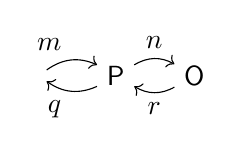
\begin{tikzpicture}[baseline=(O.base)]
    \node (I) at (0,0) {};
    \node (P) at (1,0) {\kw{P}};
    \node (O) at (2,0) {\kw{O}};
    \path [->] (I) edge[bend left] node[auto] {$m$} (P);
    \path [->] (P) edge[bend left] node[auto] {$n$} (O);
    \path [->] (P) edge[bend left] node[auto] {$q$} (I);
    \path [->] (O) edge[bend left] node[auto] {$r$} (P);
  \end{tikzpicture}
  \quad
  \begin{array}{c@{\,}l@{\quad}c@{\,}l}
    m &\in M_B^\kw{Q} & q &\in M_A^\kw{Q} \\[1ex]
    n &\in M_B^\kw{A} & r &\in M_A^\kw{A}
  \end{array}
\]

The simplicity of our ``ground-level'' games
and the fact that we remain within the realm of
first-order types
makes our game model much simpler than
those typically used in the semantics of functional languages.
Nevertheless,
our model is expressive enough to model low-level components
of the kind treated in \S\ref{sec:modsem},
and many concepts inherited from traditional game semantics
remain relevant and useful.

%}}}

\subsubsection{Strategies} %{{{

Following the usual trace-based approach,
we will represent strategies as prefix-closed sets of
alternating plays.
To enforce the receptivity constraint,
we will simply leave odd-length plays out of the representation.
Taking well-bracketing into account as well,
a first approximation of the type of strategies
for the game $A \Rightarrow B$ is:
\[
  \mathcal{S}_{A \Rightarrow B} \: \approx \:
   \big\{ \sigma \subseteq
      M^\kw{Q}_B
      \big( M^\kw{Q}_A M^\kw{A}_A \big)^*
      \big( M^\kw{Q}_A \cup M^\kw{A}_B \big) \: \big| \:
      \sigma \mbox{ prefix-closed} \big\}
\]

%}}}

\subsubsection{Composition} \label{sec:sem:games:comp} %{{{

Consider two strategies
$\sigma : \mathcal{S}_{A \Rightarrow B}$ and
$\tau : \mathcal{S}_{B \Rightarrow C}$.
In the composite strategy
$\tau \circ \sigma : \mathcal{S}_{A \Rightarrow C}$,
$\sigma$ and $\tau$ interact
with each other over their common game $B$,
and with the environment over the respective games $A$ and $C$.
Note that because $\tau$ may invoke $\sigma$ multiple times,
we need to first promote $\sigma$ to a strategy $\sigma^\dagger$,
capable of answering several independent questions.
Writing $s \restriction X,Y$ for
the subsequence of $s$ consisting of the moves played in the games $X$ or $Y$,
the traditional formulation of composition
can be given as:
\[
    \tau \circ \sigma =
    \{ s \restriction {A,C} \mid
       s \restriction {A,B} \in \sigma^\dagger \wedge
       s \restriction {B,C} \in \tau \} \,.
\]

Note that composition may turn two reactive strategies
into a strategy exhibiting silent divergence.
This will happen in cases where
the two strategies only interact over the middle game ($s \in B^*$).
The formulation given above is appropriate when
silent divergence is identified with the empty interaction,
since in this case $s \restriction A,C$ will be empty.
However,
in the presence of nondeterminism,
this representation of divergence is insufficient \cite{gsnondet}.
In \S\ref{sec:sem:monad:intcomp}
we present an alternative,
operational account of strategy composition,
suitable in the context of our framework.

%}}}

\subsubsection{Nondeterminism} %{{{

Since we wish to model specifications
allowing a range of possible concrete behaviors,
we do not impose
the usual determinism requirement on strategies.
At any given point,
a strategy may allow several possible behaviors
of the system, or none,
and we will use trace containement as
the corresponding notion of refinement.

The introduction of nondeterminisim raises the question of
where divergence fit with respect to that refinement preorder.
In traditional denotational semantics,
answers to this question correspond to the variety of constructions
that can be used as powerdomains to model nondeterminism.
Thankfully,
the simplicity and operational flavor of game semantics
will allow us to treat this question in a much more
concrete and direct way. [elaborate, be more precise]

%}}}

\subsubsection{Divergence} %{{{

Identifying silent divergence with $\bot$
would allow a diverging program to refine any specification.
Instead,
from the point of view of refinement,
we wish to treat divergence as a behavior on par with others.
This means our strategy model must be extended
with an explicit representation of silent divergence.

In \cite{gsnondet},
this is accomplished by adjoining to every strategy
a set of the plays which may trigger silent divergence.
Equivalently,
we extend our model by allowing plays to contain
the special move $\Delta$ as the last move of the system.

Note that by contrast with \cite{gsnondet},
[b/c monad gives us just enough branching-time info,
we don't run into problems with unbounded nondeterminism]

%}}}

\subsubsection{Abstraction} %{{{

[Can we derive a notion of abstraction
from a prefix-closed concretization relation on traces?
We would define the associated
conretization and abstraction functions on strategies,
as well as the corresponding soundness relation]

%}}}

\subsubsection{Undefined Behaviors} %{{{

[We want the concretization of strategies to preserve $\top$,
for practical reasons
(the assembly program should be allowed to go wrong as well),
as well as theoretical ones
(concretization--abstraction Galois connexion).
To this end we introduce another terminal move $\lightning$.]

%}}}

\subsubsection{Sequential Compositionality} %{{{

[One last type of terminal move we have is a return value $v$
to be passed to another ``strategy fragment''.
For whole strategies the type of $v$ is $\varnothing$.

With this addition,
we can capture the various effects
denoted by our strategies
(interaction, nondeterminism, divergence)
into a monadic framework.
This is the \emph{interaction monad} introduced in the
remainder of this section.]

%}}}

\subsubsection{--- to add somehwere ---} %{{{

[Vardi's argument for trace semantics
as the externally observable things]

[the monadic approach gives us just enough
local/intermediate branching-time info
that we can avoid the usual problems
around unbounded nondeterminism.]

%}}}

%}}}

\subsection{The Interaction Monad}

% preamble {{{

[Say it's formalized in Coq / uses CIC as foundation]

The traditional representation of strategies as
prefix-closed sets of traces
offers many advantages:
it is simple;
the ordering properties of down-set lattices
are straightforward and well-understood;
as a trace semantics
it is well-suited as a fully abstract description
of a system's external behavior.

On the other hand,
the transition systems
used to define the semantics of CompCert languages
correspond more closely to the internal operation of the system
and lend themselves better
to operational resoning and intuition,
but phenomena such as branching and divergence
make it harder to pin down a single notion of equivalence \cite{blts}
and in some cases complicates the corresponding definitions of simulations.

The \emph{interaction monad} $\mathcal{I}_{M,N}(-)$
defined in this section offers advantages of both of these models.
Following traditional work on game semantics,
we use a simple trace model to formalize
the behavior of interactive components.
However,
the accompanying monadic structure
introduces a notion of sequential composition
which makes it possible to define strategies
in an operational way.
We present this approach in \S\ref{sec:monad:def}--\S\ref{sec:monad:int}.

[Something about simulations and abstraction in \S\ref{sec:monad:abs}]

The interaction monad
can be used to formalize various notions of alternating strategies.
In \S\ref{sec:monad:games},
we show a simple encoding of the
innocent, well-bracketed strategies
of a specific class of games,
which we will use as the foundation for
the semantic model presented in \S\ref{sec:modsem}.

%}}}

\subsection{Overview} \label{sec:monad:overview} %{{{






The interaction monad specifies
the behavior of an open system.
At any point,
the system can perform an output $m \in M$ and
wait for a subsequent input $n \in N$ from the environment.
This is modelled by the operation:
\[
    \kw{interact} : M \rightarrow \mathcal{I}_{M,N}(N) \,.
\]

Additionally,
to accomodate specifications which permit a range of possible behaviors,
the interaction monad is equipped with a complete refinement lattice.
Given $x, y : \mathcal{I}_{M,N}(A)$,
their supremum $x \sqcup y : \mathcal{I}_{M,N}(A)$
is the smallest specification that permits the behavior of either;
it can also be interpreted as non-deterministic choice
of the system.
Conversely, $x \sqcap y : \mathcal{I}_{M,N}(A)$ can be interpreted as
the largest specification requiring that $x$ and $y$ both be satisfied.
The least element $\bot$
is a specification that can never be satisfied;
the greatest element $\top$
is the specification that is always satisfied ---
or represents a computation whose behavior is entierely undefined.

Finally,
we model non-deterministic iteration with the operator:
\[
     -^\infty : (A \rightarrow \mathcal{I}_{M,N}(A)) \rightarrow
                (A \rightarrow \mathcal{I}_{M,N}(A)) \,.
\]
Notably,
$-^\infty$ is different from
the Kleene star associated with the refinement lattice,
because we account for silent divergence as a specific behavior,
incomparable with terminating ones,
rather than identifying it with
the unsatisfiable specification $\bot$
or the undefined behavior $\top$.

%}}}

\subsection{Definition} \label{sec:monad:def} %{{{

Following the traditional game semantics approach,
we formalize interactive behaviors as prefix-closed sets of traces.
We restrict our focus to
alternating games which do not put any restriction on $\kw{O}$,
so the traces we will consider are odd-length sequences of moves
representing the interaction between the system and the environment.
To support the monadic structure and account
for silent divergence and undefined behaviors,
we augment the set of outputs with the
distinguished terminal moves $v \in X$, $\Delta$, and $\lightning$:
\[
    s, t \in
    \mathcal{T}_{M,N}(X) ::=
    v \mid \Delta \mid \lightning \mid m \mid mnt \,.
\]
Any trace is considered a prefix of $\lightning$,
so that our extended prefix relation on $\mathcal{T}_{M,N}(X)$
is defined by the rules:
\begin{gather*}
  v \sqsubseteq v , \quad
  \Delta \sqsubseteq \Delta , \quad
  t \sqsubseteq \lightning , \quad
  m \sqsubseteq m , \quad
  m \sqsubseteq mnt ,
  \quad
  \AxiomC{$s \sqsubseteq t$}
  \UnaryInfC{$mns \sqsubseteq mnt$}
  \DisplayProof
\end{gather*}
An interactive behavior is
a prefix-closed set of traces:
\[
    \mathcal{I}_{M,N}(X) :=
    \{ T \subseteq \mathcal{T}_{M,N}(X) \mid
       \forall t \in T \,.\, \forall s \sqsubseteq t \,.\, s \in T \}
\]

Note that since any trace is a prefix of $\lightning$,
a behavior which admits a trace ending with $\lightning$
will also admit all possible interactions
sharing the same initial segment.
This allows us to define our notion of refinement
as simple trace containment.
For $x, y \in \mathcal{I}_{M,N}(X)$, refinement is defined as:
\[
    x \sqsubseteq y \Leftrightarrow x \subseteq y
\]
Since unions and intersections
preserve prefix closure,
they induce a lattice structure on $\mathcal{I}_{M,N}(X)$.

%}}}

\subsection{Monad operations} %{{{

The monad's unit associates to each value $v \in X$
the computation with a single trace $v$:
\[
    \kw{ret}_X(v) := \{ v \} \,.
\]
The binding operation corresponds to
the sequential composition of
a behavior $x \in \mathcal{I}_{M,N}(A)$ and
a function $f : A \rightarrow \mathcal{I}_{M,N}(B)$.
The result is an interactive behavior in $\mathcal{I}_{M,N}(B)$ which
contains the traces of $x$ where
any final value $v$ has been replaced with
all possible traces in $f(v)$.
For a single trace $t \in x$ we define $t \bind f$
using the following rules:
\begin{gather*}
  \AxiomC{}
  \UnaryInfC{$\Delta \in (\Delta \bind f)$}
  \DisplayProof
  \quad
  \AxiomC{}
  \UnaryInfC{$t \in (\lightning \bind f)$}
  \DisplayProof
  \quad
  \AxiomC{}
  \UnaryInfC{$m \in (m \bind f)$}
  \DisplayProof
  \\[1ex]
  \AxiomC{$t \in f(v)$}
  \UnaryInfC{$t \in (v \bind f)$}
  \DisplayProof
  \quad
  \AxiomC{$s \in (t \bind f)$}
  \UnaryInfC{$mns \in (mnt \bind f)$}
  \DisplayProof
\end{gather*}
Then $x \bind f$ can be defined as:
\[
    (x \bind f) = \bigcup_{t \in x} (t \bind f)
\]
It is straightforward to verify that
the monad laws hold:
\begin{align*}
  (\kw{ret}(v) \bind f) &= f(v) \\
  (x \bind \kw{ret}) &= x \\
  (x \bind (v \mapsto f(v) \bind g)) &= ((x \bind f) \bind g) \,.
\end{align*}

While interactive behaviors $x : \mathcal{I}_{M,N}(A)$
represent active computations,
the monad's Kleisli morphisms $f : A \rightarrow \mathcal{I}_{M,N}(B)$
can be interpreted as \emph{interactive continuations}:
suspended computations which can be resumed by an input $v : A$.
Kleisli morphisms can be used to
model strategies for games in which $\kw{O}$ plays first,
as demonstrated in \S\ref{sec:monad:games}.
In addition,
a Kleisli morphism
$f : A \rightarrow \mathcal{I}_{M,N}(A)$
with identical argument and result types
can be interpreted as an \emph{interactive transition system},
as demonstrated in \S\ref{sec:monad:powerset}.

The binding operation $\bind$
and the lattice structure on $\mathcal{I}_{M,N}(A)$
can be extended to Kleisli morphisms as follows:
\begin{align*}
    (f \cdot g)(a) &:= f(a) \bind g &
    \mathbf{1}(a) &:= \kw{ret}(a) \\
    (f \oplus g)(a) &:= f(a) \sqcup g(a) &
    \mathbf{0}(a) &:= \bot
\end{align*}
Together with the iteration principles
defined in the following section,
these operations constitute a structure
analogous to a typed Kleene algebra \cite{tka}.

%}}}

\subsection{Iteration} \label{sec:monad:iter} %{{{

A Kleisli morphism $f : A \rightarrow \mathcal{I}_{M,N}(A)$
can be iterated as follows.
We start by defining
the $n$-fold sequential composition of $f$
and the associated notion of Kleene star as:
\begin{align*}
    f^0(a) &:= \kw{ret}(a) \\
    f^{n+1}(a) &:= f^n(a) \bind f \\
    f^*(a) &:= \bigsqcup_n f^n(a) \,.
\end{align*}
In order to recognize silent divergence,
we introduce $f_\Delta$,
defined by the following coinductive rule.
Note that $f_\Delta(v) \sqsubseteq \{\Delta\}$.
\[
    \AxiomC{$v' \in f(v)$}
    \AxiomC{$\Delta \in f_\Delta(v')$}
    \doubleLine
    \BinaryInfC{$\Delta \in f_\Delta(v)$}
    \DisplayProof
\]
Then the non-deterministic, infinite iteration of $f$ is:
\[
    f^\infty := (f \oplus f_\Delta)^*
\]

%}}}

\subsection{Sets and Functions} \label{sec:monad:powerset} %{{{

The powerset monad $\mathcal{P}$
can be embedded into the monad $\mathcal{I}_{M,N}$
using the natural transformation
$\eta^\mathcal{P}_X : \mathcal{P}(X) \rightarrow \mathcal{I}_{M,N}(X)$
defined as:
\[
    \eta^\mathcal{P}_X(V) := \{ v \mid v \in V \}
\]
In particular,
a relation $R : A \rightarrow \mathcal{P}(B)$
can be interpreted as
$\eta^\mathcal{P}_B \circ R : A \rightarrow \mathcal{I}_{M,N}(B)$.

\begin{example} \label{ex:ts} % Transition system {{{
Consider a transition system $\alpha = (S, I, {\rightarrow}, F)$,
where
$S$ is a set of states,
$I : \mathcal{P}(S)$
is a set of initial states,
${\rightarrow} : S \rightarrow \mathcal{P}(S)$
is a transition relation, and
$F : S \rightarrow \mathcal{P}(A)$
associate potential output values to each state.
The behavior of $\alpha$ can be expressed as:
\[
    \llbracket \alpha \rrbracket :=
    \eta^\mathcal{P}_S(I) \bind
    (\eta^\mathcal{P}_S \circ {\rightarrow})^\infty \bind
    (\eta^\mathcal{P}_S \circ F)
    : \mathcal{I}_{M,N}(A) \,.
\]
\end{example}
%}}}

We use a similar pattern in \S\ref{sec:modsem:def}
to express the behavior of CompCert small-step semantics
in terms of interactive behaviors.
For conciseness,
we will sometimes rely implicitly on $\eta_X^\mathcal{P}$
when a set $x : \mathcal{P}(A)$ is used
in a context where an interactive behavior
of type $\mathcal{I}_{M,N}(A)$ is expected,
for instance expressing $\llbracket \alpha \rrbracket$ above as
$I \bind {\rightarrow}^\infty \bind F$.

Given a function $f : A \rightarrow B$,
its \emph{preimage}
$f^{-1} : B \rightarrow \mathcal{I}_{M,N}(A)$
can be defined as:
\[
    f^{-1}(b) = \eta^\mathcal{P}_A(\{ a \mid f(a) = b \}) \,.
\]
For instance, given two Kleisli morphisms
$f : A \rightarrow \mathcal{I}_{M,N}(X)$ and
$g : B \rightarrow \mathcal{I}_{M,N}(X)$,
their copairing $[f, g] : A + B \rightarrow \mathcal{I}_{M,N}(X)$
in the Kleisli category can be expressed as
$(i_1^{-1} \cdot f) \oplus (i_2^{-1} \cdot g)$.

For the sake of symmetry we will sometimes implicitly promote
$f : A \rightarrow B$ to the Kleisli morphism
$\kw{ret} \circ f : A \rightarrow \mathcal{I}_{M,N}(B)$.

%}}}

\subsection{Interaction} \label{sec:monad:int} %{{{

The interaction primitive
$\kw{interact} : M \rightarrow \mathcal{I}_{M,N}(N)$
can be defined as follows:
\[
    \kw{interact}(m) := \{ m, mnn \mid n \in N \}
\]
Note that in the trace $mnn$,
the first occurence of $n$ denotes an input,
whereas the second one denotes the value returned by $\kw{interact}$.

To eliminate interaction,
we can use the the following operator to
``silently unfold'' the next action of a behavior $x$:
\[
    \kw{next} :
       \mathcal{I}_{M,N}(X) \rightarrow
       \mathcal{I}_{P,Q}(X + M \times (N \rightarrow \mathcal{I}_{M,N}(X)))
\]
When $x$ diverges or goes wrong, so does $\kw{next}(x)$.
If $x$ returns a value $a$, then $\kw{next}(x)$ behaves as:
\[
    \kw{next}(\kw{ret}(a)) = \kw{ret}(i_1(a))
\]
However,
if $x$ attempts to interact,
then $\kw{next}(x)$ will instead
return the corresponding output $m \in M$,
as well as a continuation $N \rightarrow \mathcal{I}_{M,N}(X)$
which can be used to resume the evaluation of $x$
on a subsequent input $n \in N$:
\[
    \kw{next}(\kw{interact}(m) \bind f) = \kw{ret}(i_2(m, f)) \,.
\]

\begin{definition}[Silent unfolding]
For an interactive behavior $x : \mathcal{I}_{M,N}(A)$,
the behavior $\kw{next}(x)$ is defined by the rules:
\begin{gather*}
    \AxiomC{$v \in x$}
    \UnaryInfC{$i_1(v) \in \kw{next}(x)$}
    \DisplayProof
    \quad
    \AxiomC{$\Delta \in x$}
    \UnaryInfC{$\Delta \in \kw{next}(x)$}
    \DisplayProof
    \quad
    \AxiomC{$\lightning \in x$}
    \UnaryInfC{$\lightning \in \kw{next}(x)$}
    \DisplayProof
    \\[1ex]
    \AxiomC{$m \in x$}
    \UnaryInfC{$i_2(m, n \mapsto \delta_{mn}(x)) \in \kw{next}(x)$}
    \DisplayProof
\end{gather*}
where $\delta_{mn}(x) := \{ t \mid mnt \in x \}$.
\end{definition}

Interaction introduces a second notion of composition
besides the one induced by the $\bind$ operator:
given
$x : \mathcal{I}_{M,N}(A)$ and
$f : M \rightarrow \mathcal{I}_{P,Q}(N)$,
the behavior $x[f] : \mathcal{I}_{P,Q}(A)$
will proceed according to $x$,
but whenever $x$ attempts to perform an output $m \in M$,
the behavior $f(m)$ will be substituted;
if $f(m)$ returns a value $n \in N$,
the value will be used as an input to resume to evaluation of $x$.

Note that $x[f]$ may introduce silent divergence;
for instance:
\[
    \kw{interact}^\infty(*) [\kw{ret}] = \{ \Delta \} \,,
\]
even though neither $\kw{interact}^\infty(*)$
nor $\kw{ret}$ silently diverge on their own.
To formulate the definition of $x[f]$,
we will use an interactive transition system
based on $\kw{next}$,
over states of type $\mathcal{I}_{M,N}(A) + A$.
A state $i_1(\hat{x})$ denotes that
the evaluation of $x$ is still active,
with $\hat{x}$ the remaining suffix of its behavior.
A state $i_2(v)$ denotes that
$x$ has terminated with the result $v$.

\begin{definition}[Substitution]
For a type $A$ and
an interactive continuation $f : M \rightarrow \mathcal{I}_{P,Q}(N)$,
we define
$\vec{f}_A : \mathcal{I}_{M,N}(A) + A \rightarrow
 \mathcal{I}_{P,Q}(\mathcal{I}_{M,N}(A) + A)$
as the interactive transition system:
\begin{align*}
  \vec{f}_A(s) := i_1^{-1}(s) \bind \kw{next} \bind
      [i_2, (m, k) \mapsto f(m) \bind n \mapsto \kw{ret}(i_1(k(n)))]
%        (&i_1^{-1} \bind i_2) \\ {} \oplus
%        (&i_2^{-1} \bind (m, k) \mapsto f(m) \bind k \bind i_1)
\end{align*}
Then for a behavior $x : \mathcal{I}_{M,N}(A)$,
the \emph{substitution} $x[f] : \mathcal{I}_{P,Q}(A)$ is defined as:
\[
    x[f] := \kw{ret}(i_1(x)) \bind \vec{f}_A^\infty \bind i_2^{-1} \,,
\]
and for $g : A \rightarrow \mathcal{I}_{M,N}(B)$,
the \emph{interactive composition}
$g \odot f : A \rightarrow \mathcal{I}_{P,Q}(B)$ is defined as:
\[
    (g \odot f)(a) := g(a) [f] \,.
\]
\end{definition}

Substitution and interactive composition
enjoy the following properties:
\begin{align*}
  x[\kw{interact}] &= x &
  \kw{interact}(m)[f] &= f(m) &
  x[g \odot f] &= x[g][f] \\
  g \odot \kw{interact} &= g &
  \kw{interact} \odot f &= f &
  h \odot (g \odot f) &= (h \odot g) \odot f
\end{align*}

In addition,
similarly to the way
the Kleene composition $f \cdot g$ can be iterated as $f^\infty$,
we can let a behavior interact with itself
by iterating the interactive composition $f \odot g$ as $f^\oast$.
For $f : M \rightarrow \mathcal{I}_{M,N}(N)$,
The transition system used to defined $f^\oast$
uses states of type $(N \rightarrow \mathcal{I}_{M,N}(N)$

\begin{definition}[Interactive iteration]
[A bit more involved because we need to keep a stack of continuations.
Maybe define in terms of traces if that's more transparent.]
\end{definition}

[Rename $\kw{interact}$ as $\mathbf{I}$
given that it is the identity for $\odot$?]

%}}}

\subsection{Abstraction} \label{sec:monad:abs} %{{{

We now consider the problem of relating interactive behaviors
whose inputs, outputs, and results are taken in different sets.
We will use Kripke logical relations to relate these components,
so that the correspondance between the two interactions
can be sensitive to the history of the computation.

\begin{definition}
For sets of inputs $M_1, M_2$, outputs $N_1, N_2$, and results $X_1, X_2$,
a \emph{simulation convention} between them
is a tuple $\mathbb{R} = \langle W, \leadsto, R_M, R_N, R_X \rangle$
where $\langle W, \leadsto \rangle$ is a Kripke frame, and
$R_M : \mathcal{R}_W(M_1, M_2)$,
$R_N : \mathcal{R}_W(N_1, N_2)$,
$R_X : \mathcal{R}_W(X_1, X_2)$
are $W$-indexed Kripke logical relations
between the respective sets of inputs, outputs and results.
\begin{itemize}
\item
The identity simulation convention is defined as
$\mathbbm{1} := \langle \{*\}, \{(*,*)\}, {=}, {=}, {=} \rangle$.
\item
The composition of
the simulation conventions $\mathbb{R}$ and $\mathbb{S}$ is:
\[
    \mathbb{R} \cdot \mathbb{S} :=
      \langle
        W_\mathbb{R} \times W_\mathbb{S}, \:
        {\leadsto}_\mathbb{R} \times {\leadsto}_\mathbb{S}, \:
        R_M \cdot S_M, \:
        R_N \cdot S_N, \:
        R_X \cdot S_X
      \rangle \,,
\]
where $R \cdot S$ denotes the Kripke relation defined by:
\[
    (w_1, w_2) \Vdash R \cdot S \: := \:
      (w_1 \Vdash R) \cdot (w_2 \Vdash S) \,.
\]
\item
Given two simulation conventions
$\mathbb{R} = \langle W, \leadsto, R_M, R_N, R_V \rangle$ and
$\mathbb{R}' = \langle W', \leadsto, R_M', R_N', R_V' \rangle$,
we say that $\mathbb{R}$ \emph{refines} $\mathbb{R}'$
and write $\mathbb{R} \sqsubseteq \mathbb{R}'$
when:
\begin{align*}
  \forall w \in W \,.\, (
    &\forall (v_1, v_2) \in [w \Vdash R_V] \,.\, \\
    &\exists w' \in W' \,.\, (v_1, v_2) \in [w' \Vdash R_V']) \\
  \wedge \: (
    &\forall (m_1, m_2) \in [w \Vdash R_M] \,.\, \\
    &\exists w' \in W' \,.\, (m_1, m_2) \in [w' \Vdash R_M'] \: \wedge \\
    &\forall v' \in W' \,.\, w' \leadsto v' \Rightarrow \\
    &\forall (n_1, n_2) \in [v' \Vdash R_N'] \,.\, \\
    &\exists v \,.\, w \leadsto v \wedge (n_1, n_2) \in [v \Vdash R_N] )
\end{align*}
\end{itemize}
\end{definition}

Simulation conventions relate interactions which have the same \emph{shape},
in the sense that there is a one-to-one correspondance between
the inputs and outputs of $x_1$ and $x_2$.
Nevertheless,
extending a simulation convention $\mathbb{R}$ to behaviors
is complicated by the alternating roles of the system and the environment.
Our goal will be to define a Kripke relator:
\[ {\le}_\mathbb{R} \: = \:
   \mathcal{I}^\le_{R_M,R_N}(R_X) \: : \:
   \mathcal{R}_W(\mathcal{I}_{M_1,N_1}(X_1), \mathcal{I}_{M_2,N_2}(X_2)) \]
such that $x_1 \le_\mathbb{R} x_2$
whenever $x_1$ is simulated by $x_2$ according to $\mathbb{R}$.
We will proceed by defining a mapping:
\[ \mathbb{R}^*_w : \mathcal{I}_{M_2,N_2}(X_2) \rightarrow
                    \mathcal{I}_{M_1,N_1}(X_1) \, \]
such that $\mathbb{R}^*_w(x_2)$ is
the largest computation in $\mathcal{I}_{M_1,N_1}(X_1)$
simulated by $x_2$.
Accordingly,
we will define:
\[ w \Vdash x_1 \le_\mathbb{R} x_2 \: \Leftrightarrow \:
   x_1 \sqsubseteq \mathbb{R}^*_w(x_2) \,. \]

In the presence of different levels of abstraction
related by a convention $\mathbb{R}$,
the mapping $\mathbb{R}^*$ will allow us to embed a high-level specification
into a low-level semantic domain
where it can be compared with
the concrete behavior of the system we seek to verify.
In a complementary way, $\le_\mathbb{R}$
allows us to express abstraction relationally;
specifically, the primitives of the interaction monad
will enjoy properties with respect to $\le_\mathbb{R}$
which will help us construct
simulations between
structurally similar computations
operating at different levels of abstraction.

\begin{definition}
For a simulation convention $\mathbb{R} = \langle R_M, R_N, R_X \rangle$
and a behavior $x_2 : \mathcal{I}_{M_2, N_2}(X_2)$,
the behavior $\mathbb{R}^*_w(x_2)$ is defined by the rules:
\begin{gather*}
  \AxiomC{$v_2 \in x_2$}
  \AxiomC{$v_1 \ifr{w \Vdash R_X} v_2$}
  \BinaryInfC{$v_1 \in \mathbb{R}^*_w(x_2)$}
  \DisplayProof
  \qquad
  \AxiomC{$\Delta \in x_2$}
  \UnaryInfC{$\Delta \in \mathbb{R}^*_w(x_2)$}
  \DisplayProof
  \qquad
  \AxiomC{$\lightning \in x_2$}
  \UnaryInfC{$t \in \mathbb{R}^*_w(x_2)$}
  \DisplayProof
  \\[1ex]
  \AxiomC{$m_2 \in x_2$}
  \AxiomC{$w \leadsto w'$}
  \AxiomC{$m_1 \ifr{w' \Vdash R_M} m_2$}
  \TrinaryInfC{$m_1 \in \mathbb{R}^*_w(x_2)$}
  \DisplayProof
  \\[1ex]
  \AxiomC{$
    \begin{array}{c}
      m_2 \in x_2 \qquad
      w \leadsto w' \qquad
      m_1 \ifr{w' \Vdash R_M} m_2
      \\[.3ex]
      \forall \: w'' \, n_2 \:.\:
        w' \leadsto w'' \: \wedge \:
        n_1 \ifr{w'' \Vdash R_N} n_2 \: \Rightarrow \:
        t_1 \in \mathbb{R}^*_{w''}(\delta(x_2, m_2)(n_2))
    \end{array}$}
  \UnaryInfC{$m_1 n_1 t_1 \in \mathbb{R}^*_w(x_2)$}
  \DisplayProof
\end{gather*}
\end{definition}

The mapping $\mathbb{R}^*$ preserves our constructions
on simulation conventions in the following ways:
\begin{gather*}
\mathbbm{1}^*_w(x) = x \\
(\mathbb{R} \cdot \mathbb{S})^* = \mathbb{S}^* \circ \mathbb{R}^* \\
-^* : {\sqsubseteq} \rightarrow {\sqsubseteq} \rightarrow {\sqsubseteq}
\end{gather*}
These properties ensure that
the relational version of $\mathbb{R}^*$,
defined below as $\le_\mathbb{R}$,
behaves as a relator.

\begin{definition}
For a simulation convention $\mathbb{R} = \langle R_M, R_N, R_X \rangle$,
a world $w$,
and two interactive behaviors
$x_1 : \mathcal{I}_{M_1, N_1}(X_1)$ and
$x_2 : \mathcal{I}_{M_2, N_2}(X_2)$,
we say that
\emph{$x_1$ is simulated at $w$ by $x_2$ according to $\mathbb{R}$}
and write:
\[
    x_1 \ifr{w \Vdash {\le}_\mathbb{R}} x_2
    \quad \mbox{or} \quad
    x_1 \ifr{w \Vdash \mathcal{I}^\le_{R_M,R_N}(R_X)} x_2
\]
whenever $x_1 \sqsubseteq \mathbb{R}^*_w(x_2)$.
\end{definition}

Whenever possible,
for brevity's sake we will use the notation $\le_\mathbb{R}$.
When we need to make the components relations of $\mathbb{R}$ explicit,
we will use the notation $\mathcal{I}_{R_M,R_N}(R_X)$ instead.

Identity and composition yield
${\le}_\mathbbm{1} = {\sqsubseteq}$ and
${\le}_{\mathbb{R} \cdot \mathbb{S}} =
 {\le}_\mathbb{R} \cdot {\le}_\mathbb{S}$.
More generally,
the following properties make
$\le_\mathbb{R}$ a \emph{relator} \cite{something}:
\begin{align*}
  {=} &\subseteq {\le}_\mathbbm{1} \\
  {\le}_{\mathbb{R} \cdot \mathbb{S}} &\subseteq
    {\le}_\mathbb{R} \cdot {\le}_\mathbb{S} \\
  \mathbb{R} \sqsubseteq \mathbb{S} &\Rightarrow
    {\le}_\mathbb{R} \subseteq {\le}_\mathbb{S}
\end{align*}
In particular, $\le_\mathbb{R}$ is compatible with $\sqsubseteq$
in the following sense:
\[
    {\sqsubseteq} \cdot {\le}_\mathbb{R} =
    {\le}_\mathbb{R} \cdot {\sqsubseteq} =
    {\le}_\mathbb{R}
\]

We can now formulate the following properties,
which describe the behavior of the monad's primitives
with respect to abstraction and refinement:
\begin{align*}
  \kw{ret} &:
    {}\Vdash R_X \rightarrow \mathcal{I}^\le_{R_M,R_N}(R_X) \\
  \bind &:
    (\Vdash R_X \rightarrow
     \mathcal{I}^\le_{R_M,R_N}(R_Y)) \rightarrow
    (\Vdash \mathcal{I}^\le_{R_M,R_N}(R_X) \rightarrow
     \mathcal{I}^\le_{R_M,R_N}(R_Y)) \\
  \kw{interact} &:
    (\Vdash (\Diamond R_M) \rightarrow
     \mathcal{I}^\le_{R_M,R_N}(R_N)) \\
  \kw{next} &:
    (\Vdash \mathcal{I}^\le_{R_M,R_N}(R_X) \rightarrow
     R_X +
     \Diamond (R_M \times
     \Box (R_N \rightarrow \mathcal{I}^\le_{R_M,R_N}(R_X)))) \\
  -^\infty &:
    (\Vdash R_X \rightarrow \mathcal{I}^\le_{R_M,R_N}(R_X)) \rightarrow
    (\Vdash R_X \rightarrow \mathcal{I}^\le_{R_M,R_N}(R_X)) \\
  \eta^\mathcal{P} &:
    (\Vdash \mathcal{P}^\le(R_X) \rightarrow
     \mathcal{I}^\le_{R_M,R_N}(R_X))
\end{align*}
Together,
these properties allow us to construct
heterogenous simulations
between monadic terms with similar structures.

\begin{example} \label{ex:sim}
Building on our previous example,
consider
$\alpha_1 = (S_1, I_1, {\rightarrow}_1, F_1)$ and
$\alpha_2 = (S_2, I_2, {\rightarrow}_2, F_2)$
two transition systems,
together with a relation
$R : \mathcal{R}(S_1, S_2)$
satisfying:
\begin{gather*}
  I_1 \ifr{\mathcal{P}^\le(R)} I_2 \\
  {\rightarrow}_1 \ifr{R \rightarrow \mathcal{P}^\le(R)} {\rightarrow}_2 \\
  F_1 \ifr{R \rightarrow \mathcal{P}^\le(=)} F_2
\end{gather*}
That is, $R$ is a simulation relation between $\alpha_1$ and $\alpha_2$.
Then by using the properties above and
following the structure of $\llbracket - \rrbracket$,
we can show that:
\[
    \llbracket \alpha_1 \rrbracket \sqsubseteq
    \llbracket \alpha_2 \rrbracket \,.
\]
\end{example}

%}}}

\subsection{Games and Strategies} \label{sec:monad:games} %{{{

[Just define our notion of elementary game / language interface,
and the notion of strategy for $A \Rightarrow B$
that we will use for CompCert semantics.
Connect to HON games]

[For now let's note that we will write $\sigma : A \Rightarrow B$
whenever
$\sigma : M_B^\kw{Q} \rightarrow
\mathcal{I}_{M_A^\kw{Q}, M_A^\kw{A}}(M_B^\kw{A})$.]

%}}}

%}}}

\section{Semantics of CompCert Modules} \label{sec:modsem} %{{{

% preamble {{{

Having laid out our basic semantic framework,
we now use it to construct a compositional semantic model
for open modules in CompCert.

%}}}

\subsection{Overview} %{{{

CompCert is a C-to-assembly compiler written and verified
in the Coq proof assistant.
The compiler is accompanied by
a formal semantics of the source, target, and intermediate languages,
and a proof that if the compiler succeeds,
then the behavior of the emitted target program
refines that of the source program.

The semantics of CompCert languages
are given as labeled transition systems (LTS)
modeling the execution of a whole program's \texttt{int main()} function.
The semantics of external calls
is a global parameter common to all languages,
and may use a fixed set of actions as a rudimentary model
of the program's interaction with the environment.
The externally observable behavior of the program
is given by defining the set of traces associated with any LTS,
and the various kinds of simulations used by CompCert
are shown to be sound with respect to trace containement.

CompCert, however,
does not attempt to model the semantics of open modules,
nor to define a semantic notion of module composition.
We achive this using the following approach:
\begin{itemize}
\item Following Compositional CompCert \cite{compcompcert},
  we modify CompCert's LTS model
  to explicitely account for the two-way interaction
  between a program module and its environment
  in terms of control transfers associated with
  function calls and returns.
\item We generalize this model further by
  using elementary games to parametrize the LTS model, and
  using refinement conventions to parametrize
  CompCert's notions of simulations.
  Games specify the form of function calls and returns,
  whereas refinement conventions serve to express
  generalized calling conventions between the various
  languages involved in the compilation process.
\end{itemize}

In \S\ref{sec:modsem:def},
we introduce our changes to CompCert's LTS model,
and define their behavior in terms of interactive computations.
In \S\ref{sec:modsem:ref},
we carry out those changes to the notions of
forward and backward simulations
present in CompCert,
and show them sound with respect to refinement.
In \S\ref{sec:modsem:comp},
[composition].
[Figure out how abstraction fits in].

%}}}

\subsection{Definition} %{{{
\label{sec:modsem:def}

The semantics of CompCert languages are given mainly
as labeled transition systems (LTS).
In the original CompCert,
a labeled transition system is given as
a set of states $S$,
a subset $I \subseteq S$ of initial states,
a labeled transition relation
${\rightarrow} \subseteq S \times \mathbb{E}^* \times S$,
and a set
$F \subseteq S \times \kw{int}$
of final states associated with integer results.
Compcert LTS support a notion of interaction with the environment
in the form of event traces:
a transition $s \stackrel{t}{\rightarrow} s'$,
indicates that the state $s$ may transition to state $s'$
through an interaction recorded as the event trace $t \in \mathbb{E}^*$.

For the range of languages that we are considering
($\kw{Clight}$--$\kw{Asm}$),
non-empty event traces are only generated by
the predefined semantics of external calls.
Since this model is insufficient to express
the semantics of open C and assembly modules,
we replace this facility with
and explicit treatment of incoming and outgoing calls
at the level of transition systems.

\begin{definition}[Small-step semantics]
Given two elementary games $A, B$,
a \emph{small-step semantics} for the game $A \Rightarrow B$
is a tuple $L = \langle S, \rightarrow, I, X, Y, F \rangle$.
$S$ is a set of states,
with ${\rightarrow} \subseteq S \times S$ a \emph{transition relation} on $S$.
The handling of incoming calls is specified by
$I \subseteq M_B^\kw{Q} \times S$, which
assigns a set of \emph{initial states} to each question of $B$, and
$F \subseteq S \times M_B^\kw{A}$,
which designates \emph{final states} together with corresponding answers.
The handling of external calls is specified by
$X \subseteq S \times M_A^\kw{Q}$,
which identifies \emph{external states} together with
corresponding questions of $A$ directed to the environment, and
$Y \subseteq S \times M_A^\kw{A} \times S$,
which is used to select a \emph{resumption state}
based on the outcome of the external call
after the environment returns control to the module.

We write $L : \kw{semantics}(A, B)$ to indicate that
$L$ is a small-step semantics for the game $A \rightarrow B$.
\end{definition}

CompCert interprets the lack of any transition (``getting stuck'')
as undefined behavior.
This convention fits the context of
language semantics defined through inductive sets of rules:
the behavior of a state for which there are no rules is undefined.
For a small-step semantics
$L = \langle S, {\rightarrow}, I, X, Y, F \rangle : \kw{semantics}(A,B)$,
we recognize those states using the predicate:
\[
    \kw{stuck}_L(s) :=
      ({\rightarrow}(s) = \varnothing) \wedge
      (X(s) = \varnothing) \wedge
      (F(s) = \varnothing)
\]
Taking this into account,
the immediate behavior of a state $s \in S$
can be expressed as the interactive computation
$\kw{step}_L(s) : \mathcal{I}_{M_A^\kw{Q},M_A^\kw{A}}(S)$
defined as follows:
\[
  \kw{step}_L(s) :=
    \begin{cases}
      \top & \mbox{if } \kw{stuck}(s) \\
      {\rightarrow}(s) \sqcup
      (X(s) \bind \kw{interact} \bind Y(s)) & \mbox{otherwise,}
   \end{cases}
\]
The overall external behavior of $L$
can then be given as an interactive computation
$
    \llbracket L \rrbracket :
      M_B^\kw{Q} \rightarrow \mathcal{I}_{M_A^\kw{Q},M_A^\kw{A}}(M_B^\kw{A})
$
defined by:
%Then $\llbracket L \rrbracket$ can be defined as:
\begin{align*}
  \llbracket L \rrbracket (q) :=
    \begin{cases}
       \top & \mbox{if } I(q) = \varnothing \\
       I(q) \bind \kw{step}^\infty \bind F & \mbox{otherwise.}
     \end{cases}
\end{align*}

[Perhaps make this point here:
For now,
we can remark that transition systems in the form defined above
describe the behavior of a \emph{single} invocation
of the program module being modeled.
With each incoming question,
we will instantiate a new, independent state
using the initial-state predicate $I$.
The derived strategies will be innocent,
in the sense that they will not maintain
any hidden state across subsequent or reentrant
invocations from the environment.
Instead,
relevant global state will be passed back into the module
as a component of the environment's question
(for instance in the form of the memory state component
of the question as described in Table~\ref{tbl:li}).]

%}}}

\subsection{Refinement and Abstraction} %{{{
\label{sec:modsem:ref}

The correctness of CompCert is established in terms of
a \emph{backward simulation}
between the small-step semantics of the source and target programs.
In turn, backward simulations
are shown to be sound with respect to trace containement.
In this section,
we define backward simulations for our updated notion
of small-step semantics,
and show that they are sound with respect to
refinement and abstraction of interactive behaviors.

% Footnote pointing out difference w/ "Fw & Bw Sim" terminology?
A backward simulation asserts that any transition in the target program
has a corresponding transition sequence in the source program.
A transition in the target program can be matched with
an empty transition sequence in the source program;
however, to ensure the preservation of silent divergence,
this can only happen for finitely many consecutive target transitions.
This restriction is enforced by indexing the simulation relation
over a well-founded order,
and making sure that the index decreases
whenever a potentially empty sequence of source transitions is used.

In our setting,
the definition of backward simulations needs to be extended
to take into account the correspondance between
the source and target questions and answers
This can be specified using the notion of simulation convention
defined in \S\ref{sec:monad:abs}:
a simulation between the small-step semantics
$L_1 : \kw{semantics}(A_1, B_1)$ and
$L_2 : \kw{semantics}(A_2, B_2)$ will
operate in the context of the refinement convention
$\mathbb{C}_A : \mathcal{R}_{W_A}(A_1, A_2)$ and
$\mathbb{C}_B : \mathcal{R}_{W_B}(B_1, B_2)$.

Note that initial and resumption states on one hand,
and external and final states on the other hand,
correspond to respective actions of the environment and the system;
as such, they need to be treated differently.
Furthermore,
the potential non-determinism present in small-step semantics
is interpreted as \emph{system} non-determinism,
so that when relating sets of states
we will want to make sure that
each \emph{target} state has a corresponding \emph{source} state,
but the source program may allow additional behaviors
that are not realized in the target program.
This rule is slightly altered to take into account the convention that
empty sets of states correspond to undefined behaviors,
so that if the source set is empty,
no restrictions are placed on the target state.

\begin{definition}[Backward simulation between sets of states]
We say that $R : \mathcal{R}(S_1, S_2)$ is a
\emph{backward simulation relation
  between the sets $X_1 \subseteq S_1$ and  $X_2 \subseteq S_2$}
if the following conditions hold:
\begin{enumerate}
\item
  If $X_1$ is non-empty,
  then $X_2$ is non-empty as well.
\item
  If $X_1$ is non-empty,
  then for all $s_2 \in X_2$,
  there exists $s_1 \in X_1$
  such that $(s_1, s_2) \in R$.
\end{enumerate}
We will write $X_1 \ge_R X_2$.
\end{definition}

A state $s$ \emph{goes wrong}
if it is neither an external nor a final state,
and if there is no transition $s \rightarrow s'$;
a state $s$ is \emph{safe}
if no state that goes wrong is reachable from $s$
by the transition relation $\rightarrow$.
Safe states will be denoted using the predicate $\kw{safe}(s)$.
With this we are ready to define backward simulations.

\begin{definition}[Backward simulation]
Given
$\mathbb{C}_A : \mathcal{R}(A_1, A_2)$ and
$\mathbb{C}_B : \mathcal{R}(B_1, B_2)$
two simulation conventions,
and given
$L_1 : \kw{semantics}(A_1, B_1)$ and
$L_2 : \kw{semantics}(A_2, B_2)$
two small-step semantics,
a \emph{backward simulation} between $L_1$ and $L_2$
consists in a
well-founded relation $(I, <)$
together with a family of relations
$(R_i : \mathcal{R}_{W_B}(S_1, S_2))_{i \in I}$
satisfying the following properties:
\begin{description}
\item[Initial states]
  For all
  $q_1 \ifr{w \Vdash {\preceq}_B^\kw{Q}} q_2$,
  the condition $I_1(q_1) \ge_{\exists i . R_i} I_2(q_2)$ holds.
\item[External calls]
  For all $s_1 \ifr{w \Vdash R_i} s_2$
  with $s_1$ a safe state, and
  for any question $m_2 \in M_{A_2}^\kw{Q}$
  such that $(s_2, m_2) \in X_2$,
  there exists $w' \in W_A$ and $q_1 \in M_{A_1}^\kw{Q}$
  such that $q_1 \ifr{w' \Vdash {\preceq}_A^\kw{Q}} q_2$.
  In addition, for all corresponding answers
  $r_1 \ifr{w' \Vdash {\preceq}_A^\kw{A}} r_2$,
  the condition $Y_1(s_1, r_1) \ge_{\exists i . R_i} Y_2(s_2, r_2)$ holds.
\item[Final states]
  For all $s_1 \ifr{w \Vdash R_i} s_2$
  with $s_1$ a safe state, and
  for any answer $r_2 \in M_{B_2}^\kw{A}$
  such that $(s_2, r_2) \in F_2$,
  there exists a state $s_1'$ reachable from $s_1$ and
  an answer $r_1 \in M_{B_1}^\kw{A}$ such that
  $(s_1', r_1) \in F_1$ and $r_1 \ifr{w \Vdash {\preceq}_B^\kw{A}} r_2$.
\item[Progress]
  For all $s_1 \ifr{w \Vdash R_i} s_2$
  with $s_1$ a safe state,
  $s_2$ does not go wrong.
\item[Simulation]
  For all $s_1 \ifr{w \Vdash R_i} s_2$,
  if $s_1$ is a safe state and $s_2 \rightarrow s_2'$,
  then there exists $i' \in I$ and $s_1' \in S_1$
  such that $s_1' \ifr{w \Vdash R_{i'}} s_2'$ and
  such that one the following conditions hold:
  \[
    s_1 \rightarrow^+ s_1' \,, \quad \mbox{or} \quad
    s_1 \rightarrow^* s_1' \:\wedge\: i' < i \,.
  \]
\end{description}
We will write $L_1 \ge_{\mathbb{C}_A \Rightarrow \mathbb{C}_B} L_2$.
\end{definition}

[Maybe short commentary to unpack some of that.]

Stated in their full generality,
CompCert backward simulations are notably complex.
Fortunately,
many simpler formulations and related constructions
can be used to establish
the existence of backward simulations
for specific compiler passes.
However,
backward simulations are not easily amenable to
meta-theoretical analysis
where they can appear both as hypotheses and conclusions,
which is an additional motivation for introducing
our game-based framework.
In the rest of this section we show that
backward simulations between small-step semantics
are sound with respect to
our much simpler notion of refinement
over interactive behaviors.

[Do that.]

%}}}

\subsection{Composition} \label{sec:modsem:comp} %{{{

Given two semantic objects
$\sigma_1 : B \Rightarrow C$ and
$\sigma_2 : A \Rightarrow B$,
their interactive composition $\sigma_1 \odot \sigma_2 : A \Rightarrow C$,
per the definition in \S\ref{sec:monad:int},
computes the behavior of $\sigma_1$ when $\sigma_2$ is used
to interpret its external calls.
In addition,
to model cross-module interactions in low-level programs,
we define the symmetric,
\emph{horizontal composition}
of
$\sigma_1 : A \Rightarrow A$ and
$\sigma_2 : A \Rightarrow A$,
which allows $\sigma_1$ and $\sigma_2$
to interact with one another
in a mutually recursive fashion.

\begin{definition}[Horizontal composition]
For an elementary game $A$,
the \emph{horizontal composition} of the interactive behaviors
$\sigma_1, \sigma_2 : A \Rightarrow A$
is the interactive behavior
$\sigma_1 \bullet \sigma_2 : A \Rightarrow A$
defined as:
\[
    \sigma_1 \bullet \sigma_2 :=
      (\sigma_1 \oplus \sigma_2)^\oast \,.
\]
\end{definition}

The commutativity of $\bullet$ trivially follows from that of $\oplus$,
and associativity can be derived from properties of $\oplus$ and $\oast$.
The empty behavior $\mathbf{0}$ and
the ``pass-through'' behavior $\kw{interact}$
are both identities for $\bullet$.
In addition,
the following approximations that can be useful for proofs:
\[
    \sigma_1 \odot \sigma_2 \quad \sqsubseteq \quad
    \sigma_1 \odot (\sigma_2 \oplus \kw{interact}) \quad \sqsubseteq \quad
    \sigma_1 \bullet \sigma_2 \,.
\]

%}}}

\subsection{Hiding} %{{{

Note that
in the behavior $\sigma_1 \bullet \sigma_2$,
cross-component calls remain observable:
while the external calls of $\sigma_1$
can be resolved to behaviors implemented in $\sigma_2$
(and conversely),
the original external calls remain
as non-deterministic alternatives in the final result.
[Only way to ensure associativity
because nothing prevents other components
to \emph{also} implement these functions,
in which case eliminating the calls
would make the result sensitive to the order of composition.]

This phenomenon is reminiscent of a similar one observed
in the process calculus CCS \cite{ccs}
in the context of \emph{parallel composition}.
Following this precedent,
we then define a separate \emph{hiding} operator
which retains only the external calls
which belong to a given set.

\begin{definition}[Hiding]

\end{definition}

%}}}

\subsection{Multi-module programs} %{{{

[Following composition + hiding in the last section,
extend semantic model to include component domains and/or range
and construct a notion of composition with built-in hiding
that is nevertheless associative.
Build corresponing syntactic notation
for multi-module programs.]

[Alt., syntactic linking]

%}}}

%}}}

\section{Compiler Correctness} \label{sec:compcert} %{{{

In the previous section
we have shown how to extend
the semantic model used by CompCert
to describe the behavior of open modules.
In this section
we show how the correctness proof of CompCert
can be updated to account for this additional structure.

\subsection{Overview} %{{{

Based on the existing CompCert semantics,
we will define the elementary games
$\mathcal{C}$ and $\mathcal{A}$
describing how C and assembly modules
interact with their respective environments.
The semantics of CompCert $\kw{Clight}$ and $\kw{Asm}$ programs
can then be expressed as interactive behaviors of types:
\[
    \kw{Clight} \llbracket p_s \rrbracket :
      \mathcal{C} \Rightarrow \mathcal{C} \,, \qquad
    \kw{Asm} \llbracket p_t \rrbracket :
      \mathcal{A} \Rightarrow \mathcal{A} \,.
\]
We will show that there exists a simulation convention
$\mathbb{R} : \mathcal{A} \Leftrightarrow \mathcal{C}$
such that whenever $p_t = \kw{CompCert}(p_s)$,
the following refinement property holds:
\begin{equation}
    \label{eqn:correctness}
    \kw{Asm} \llbracket p_t \rrbracket
    \, \sqsubseteq_{\mathbb{R} \Rightarrow \mathbb{R}}
    \kw{Clight} \llbracket p_s \rrbracket
\end{equation}

In Compositional CompCert,
this is achieved independently for each compilation pass.
Stated in our terms,
Compositional CompCert's \emph{interaction semantics}
employ a fixed interface $\mathcal{C}$,
and \emph{structured injections} define a single refinement convention
$\mathbb{S} : \mathcal{C} \Leftrightarrow \mathcal{C}$.
A theorem similar to (\ref{eqn:correctness}) is proved for each pass,
and structured injections are show to compose
($\mathbb{S} \cdot \mathbb{S} \equiv \mathbb{S}$),
so that a simulation theorem can be derived for the whole compiler.

A major challenge encountered in this context
is the asymmetry of requirements vs. guarantees
present in the existing proofs:
while CompCert imposes strong requirements
on the semantics of external functions,
the simulation relations used by its correctness proofs
are too weak to establish corresponding guarantees
for a module's own function executions,
preventing horizontal compositionality.
Because of this,
Compositional CompCert required significant changes
to all compilation passes,
strengthening their simulation relations
to conform to $\mathbb{S}$.

However,
our explicit treatment of abstraction
and reified notion of simulation convention
makes another approach possible.
Using existing proofs, it is reasonably straightforward
to establish a theorem of the form
for each compilation pass:
\begin{equation}
    \label{correctness-alt}
    \llbracket p_t \rrbracket
    \sqsubseteq_{\mathbb{R} \Rightarrow \mathbb{R}'}
    \llbracket p_s \rrbracket \,,
\end{equation}
where the simulation conventions $\mathbb{R}$ and $\mathbb{R}'$
characterize the assumptions and guarantees
of the existing proof.
In addition,
relevant properties of key source, target, and intermediate languages
can be expressed in relational form,
and can be used to strengthen the resulting theorem:
by composing these proofs together,
and using algebraic properties of
the simulation conventions involved,
we will be able to bridge the gap
between the domain and codomain simulation conventions
and be able to prove a correctness statement
in the form of (\ref{eqn:correctness}).

In the remainder of this section,
[dig deeper into the actual semantics and
simulation conventions used in CompCert.]
etc.

%}}}

\subsection{The CompCert Memory Model} \label{sec:compcert:mm} %{{{

\begin{figure} % fig:mm (The Compcert memory model) {{{
  \begin{gather*}
    v : \kw{val} ::=
      \kw{Vundef} \alt
      \kw{Vint}(n) \alt
      \kw{Vlong}(n) \alt
      \kw{Vfloat}(x) \alt
      \kw{Vsingle}(x) \alt
      \kw{Vptr}(b, o)
    \\
    (b, o) : \kw{ptr} :=
      \kw{block} \times \mathbb{Z}
    \\
    (b, l, h) : \kw{ptrrange} :=
      \kw{block} \times \mathbb{Z} \times \mathbb{Z}
  \end{gather*}
  \begin{align*}
    \kw{Mem.alloc} &:
      \kw{mem} \rightarrow \mathbb{Z} \rightarrow \mathbb{Z} \rightarrow
      \kw{mem} \times \kw{block}
    \\
    \kw{Mem.free} &:
      \kw{mem} \rightarrow
      \kw{ptrrange} \rightarrow
      \kw{option}(\kw{mem})
    \\
    \kw{Mem.load} &:
      \kw{mem} \rightarrow \kw{ptr} \rightarrow \kw{option}(\kw{val})
    \\
    \kw{Mem.store} &:
      \kw{mem} \rightarrow \kw{ptr} \rightarrow \kw{val} \rightarrow \kw{option}(\kw{mem})
    \\
    \kw{Mem.perm} &:
      \kw{mem} \rightarrow \kw{ptr} \rightarrow \mathcal{P}(\kw{perm})
  \end{align*}
  \caption{Outline of the Compcert memory model}
  \label{fig:mm}
\end{figure}
%}}}

The Compcert memory model \cite{compcertmmv2}
is the core algebraic structure
which underlies the semantics of Compcert's languages.
Some of its operations
are shown in Fig.~\ref{fig:mm}.
The idealized version presented here
involves
the type of memory states \kw{mem},
the types of pointers \kw{ptr} and address ranges \kw{ptrrange}, and
the type of runtime values \kw{val}.
To keep our exposition concise and clear,
we will gloss over the technical details
associated with the encoding of offsets
as concrete binary integers,
and the associated modular arithmetic and overflow constraints.
[But see artefact for the details.]

The memory is organized into a finite number of \emph{blocks}.
Each memory block has a unique identifier ($b : \kw{block}$)
represented as a positive integer,
and is equipped with its own independent linear address space.
Block identifiers and offsets are often manipulated together,
as a pair $p = (b, o) : \kw{ptr} = \kw{block} \times \mathbb{Z}$.
New blocks are created by the primitive $\kw{Mem.alloc}$,
with prescribed boundaries for their usable offsets.

A runtime value ($v : \kw{val}$) can be stored at
a given address using the primitive \kw{Mem.store},
and retreived using the primitive \kw{Mem.load}.
Values can be integers (\kw{Vint}, \kw{Vlong}) and
floating point numbers (\kw{Vfloat}, \kw{Vsingle})
of different sizes,
as well as pointers (\kw{Vptr}).
The special value \kw{Vundef}
represents an undefined value;
the simulation relations used by Compcert
usually allow $\kw{Vundef}$
to be refined into a more concrete value.

The memory model is shared by all of the languages in CompCert.
The states used to define their semantics consist of
a memory component $m : \kw{mem}$,
together with language-specific components
containing additional run-time values ($\kw{val}$).
For higher-level languages,
the language-specific component may consist of
a control stack with local environments for each activation;
for lower-level languages,
the additional component will mainly contain
the values stored in various registers.

Similarly,
our models of cross-module communication
will be built around a memory component,
accompanied by language-specific information
about function call or return events.

%}}}

\subsection{Language Interfaces} \label{sec:compcert:li} %{{{

\begin{table*} % tbl:li Language interfaces {{{
  \begin{tabular}{clll}
    \hline
    Name & Questions & Answers & Description \\
    \hline
    $\mathcal{C}$ & $(\kw{id}, \kw{sg}, \vec{v}, m)$ & $(v', m')$ &
      C-style function calls (Clight--RTL) \\
    $\mathcal{L}$ & $(\kw{id}, \kw{sg}, \kw{ls}, m)$ & $(\kw{ls}', m')$ &
      Arguments passed in abstract locations (LTL, Linear) \\
    $\mathcal{M}$ & $(\kw{id}, \kw{sp},\kw{ra},\kw{rs}, m)$ & $(\kw{rs}', m')$ &
      Arguments passed through in-memory stack (Mach) \\
    $\mathcal{A}$ & $(\kw{rs}, m)$ & $(\kw{rs}', m')$ &
      Assembly-style control transfers (Asm) \\
    \hline
  \end{tabular}
  \caption{Language interfaces for the various languages of CompCert.}
  \label{tbl:li}
\end{table*}
%}}}

The elementary games we use to model
the cross-module interactions of CompCert languages
are shown in Table~\ref{tbl:li}.
Moves correspond to control transfers
between a module and its environment:
questions correspond to function invocations;
answers return control to the caller.

At the source level ($\mathcal{C}$),
questions consist of
the name and signature of the function being invoked,
the values of its arguments,
and the state of the memory at the point of entry;
answers
consist of the function's return value
and the state of the memory at the point of exit.
This language interface is used for Clight and
for the majority of CompCert's intermediate languages.

However, starting with LTL, [...]
Once we reach Asm ($\mathcal{A}$),
queries and replies simply specify
the values of registers and the state of the memory.

%}}}

\subsection{Simulation Relations} %{{{

[Simulation relations account for refinement and abstraction,
for the change in structure between the states of different languages.
Simulation convention is the ``externally visible'' component of that.
Since core of states is mem,
core of simulation relations and conventions
are logical relation on memories.
Specific cases used in CompCert are
injections and extensions (explain).
We're going to generalize to CKLR.]

Although block identifiers and offsets
are concretely represented as integers,
there is an implicit expectation throughout CompCert
that constructions using the memory model
will not depend on specific block identities
or absolute pointer offsets.
[Explain connection to relational parametricity.]

{\color{gray} %{{{
--- [Some former material in the rest of this section:] ---

Besides equality,
the simulation proofs used
to establish the correctness of Compcert passes
relate the runtime values and memory state
that make up the states for a given language
in one of two possible ways:
memory extensions
allow the target values and memory to be more defined
than the source ones;
memory injections
additionally permits a remapping of source memory blocks
into target memory blocks at given offsets.
This remapping is specified by an injection mapping
$f : \kw{meminj}$,
where the type $\kw{meminj}$ is defined as
$\kw{block} \rightarrow \kw{option}(\kw{block} \times \mathbb{Z})$.
An entry of the form $f(b) = (b', \delta)$
signifies that the block $b$ of the source memory
is mapped into the block $b'$ of the target memory,
with offsets shifted so that
offset $0$ in $b$ will be mapped at offset $\delta$ in $b'$.

Compatibility of a given component
with extensions and injections
asserts that given two input memory states and surrounding values
in a ``memory extension'' relation
(resp. in a specific ``memory injection'' relation),
the component's outputs will preserve that relationship.
If the component allocates new memory blocks,
the injection mapping may be correspondingly extended
to introduce entries for the allocated blocks.
This is an informal description,
and the exact formulation of such theorems
vary on a component-by-component basis.
Moreover,
for many components,
CompCert needs to introduce two separate,
but very similar proofs:
one for extensions and one for injections.

As we generalize from extensions and injections
to define a family of Kripke logical relations
over the Compcert memory model,
we will be able to formalize these restrictions
in the form of unified relational parametricity theorems:
for any Compcert KLR,
such components will be related to themselves
by a relation constructed according to their type,
from the basic components provided by the KLR.
Because the KLRs are by definition compatible
with the memory model's basic operations,
such theorems will be relatively straightforward to prove,
as long as the constructions under consideration
do not access the values and memory states in exotic ways.
In addition,
because the parametricity theorems
and the properties of components
are expressed in terms of a unified relational language,
it will be possible to mechanize these proofs
to some extent.

}

%}}}

%}}}

\subsection{Kripke Logical Relations} %{{{

\begin{figure} % fig:cklr-def (Definition of CKLRs) {{{
  \begin{gather*}
    w \leadsto w \\
    w \leadsto w' \wedge w' \leadsto w'' \Rightarrow w \leadsto w'' \\
    f \ifr{(\leadsto) \rightarrow \kw{inject\_incr}} f
  \end{gather*}
  \begin{align*}
      \kw{Mem.alloc} :
        &\Vdash R^\kw{mem} \rightarrow {=} \rightarrow {=} \rightarrow
        \Diamond (R^\kw{mem} \times R^\kw{block})
      \\
      \kw{Mem.free} :
        &\Vdash R^\kw{mem} \rightarrow R^\kw{ptrrange} \rightarrow
        \kw{option}^\le(\Diamond R^\kw{mem})
      \\
      \kw{Mem.load} :
        &\Vdash R^\kw{mem} \rightarrow R^\kw{ptr} \rightarrow
        \kw{option}^\le(R^\kw{val})
      \\
      \kw{Mem.store} :
        &\Vdash R^\kw{mem} \rightarrow R^\kw{ptr} \rightarrow R^\kw{val} \rightarrow
        \kw{option}^\le(\Diamond R^\kw{mem})
      \\
      \kw{Mem.perm} :
        &\Vdash R^\kw{mem} \rightarrow R^\kw{ptr} \rightarrow {\subseteq}
  \end{align*}
  \caption{Axioms for CKLRs}
  \label{fig:cklr-def}
\end{figure}
%}}}

Memory extensions and injections
are useful for simulations
because they are specific instances
of logical relations for the CompCert memory model:
they are compatible with memory operations
in the sense that
performing similar operations on related arguments
yields related results.

\subsubsection{Definition}

We formalize this idea by defining
a notion of Kripke logical relations over the CompCert memory model,
closed under composition, and which
admits memory extensions and injections as particular instances.
As we will see,
more complex relations can also be defined,
and this will make relational parametricity theorems
particularly useful.

\begin{definition}[Compcert Kripke logical relation] \label{def:cklr} %{{{
Consider a tuple $R = (W, \leadsto, f, R^\kw{mem})$,
where
$\langle W, \leadsto \rangle$ is a Kripke frame,
$f : W \rightarrow \kw{meminj}$
associates an injection mapping to each world, and
$R^\kw{mem} : \mathcal{R}_{W}(\kw{mem})$
is a Kripke relation on memory states.
We introduce the Kripke relations
$R^\kw{ptr} : \mathcal{R}_W(\kw{ptr})$ and
$R^\kw{ptrrange} : \mathcal{R}_W(\kw{ptrrange})$
defined by the rules:
\[
  \AxiomC{$f_w(b) = (b', \delta)$}
  \UnaryInfC{$(b, o) \ifr{w \Vdash R^\kw{ptr}} (b', o + \delta)$}
  \DisplayProof
  \qquad
  \AxiomC{$(b_1, l_1) \ifr{w \Vdash R^\kw{ptr}} (b_2, l_2)$}
  \AxiomC{$h_1 - l_1 = h_2 - l_2$}
  \BinaryInfC{$(b_1, l_1, h_1) \ifr{w \Vdash R^\kw{ptrrange}} (b_2, l_2, h_2)$}
  \DisplayProof
\]
and the Kripke relation
$R^\kw{val} : \mathcal{R}_W(\kw{val})$
defined by the rules:
\begin{gather*}
  \forall \, v : \kw{val} \,.\,
    \kw{Vundef} \ifr{\Vdash R^\kw{val}} v \qquad
  \kw{Vptr} : {}
    [\Vdash R^\kw{ptr} \rightarrow R^\kw{val}] \\
  \kw{Vint}, \kw{Vlong}, \kw{Vfloat}, \kw{Vsingle} :
    [\Vdash {=} \rightarrow R^\kw{val}] \,.
\end{gather*}
We say that $R$ is a \emph{CompCert Kripke logical relation}
if the properties shown in Fig.~\ref{fig:cklr-def} are satisfied.
\end{definition}
%}}}

The $R^\kw{mem}$ component is given direcly.
We expect $R^\kw{ptr}$ to be functional
(each source pointer has at most one corresponding target pointer),
and to satisfy the following shift-invariance property:
\[
  \AxiomC{$(b_1, o_1) \ifr{R^\kw{ptr}_w} (b_2, o_2)$}
  \UnaryInfC{$(b_1, o_1 + \delta) \ifr{R^\kw{ptr}_w} (b_2, o_2 + \delta)$}
  \DisplayProof
\]
Any such relation can be uniquely specified by
an injection mapping such as $f$.
We expect the remaining components to be consistent with $R^\kw{ptr}$
and $\kw{Vundef}$ to act as a bottom element for $R^\kw{val}$.
Definition~\ref{def:cklr} follows from these conditions.

Note that $w \Vdash R^\kw{val}$
is equivalent to $\kw{Val.inject}(f_w)$
as defined in CompCert.
Furthermore, the relational property associated to $f$,
together with the definitions of
derived relations such as $R^\kw{ptr}$ and $R^\kw{val}$,
ensure that these relations are monotonic in $w$,
in the sense that:
\[
  \AxiomC{$w \leadsto w'$}
  \UnaryInfC{$R^\kw{ptr}_w \subseteq R^\kw{ptr}_{w'}$}
  \DisplayProof
  \quad
  \AxiomC{$w \leadsto w'$}
  \UnaryInfC{$R^\kw{ptrrange}_w \subseteq R^\kw{ptrrange}_{w'}$}
  \DisplayProof
  \quad
  \AxiomC{$w \leadsto w'$}
  \UnaryInfC{$R^\kw{val}_w \subseteq R^\kw{val}_{w'}$}
  \DisplayProof
\]
However,
this is not necessarily the case for $R^\kw{mem}$.

\subsubsection{Extensions}

The simplest CompCert KLR corresponds to memory extensions.
It uses a trivial Kripke frame and injection mapping:
\[
  \kw{ext} :=
    \langle \{*\}, \{(*,*)\}, * \mapsto (b \mapsto b), \kw{Mem.extends} \rangle
\]
Note that $\kw{ext}^\kw{val} = \kw{Val.inject}(b \mapsto b)$
is equivalent to $\kw{Val.lessdef}$,
which is the relation on runtime values that
CompCert uses in conjunction with \kw{Mem.extends}.

\subsubsection{Injections}

In the same vein,
we can reify memory injections as the CompCert KLR:
\[
  \kw{inj} :=
    \langle
      \kw{meminj},
      {\subseteq}, %\kw{inject\_incr},
      f \mapsto f,
      \kw{Mem.inject}
    \rangle
\]
Here the type \kw{meminj} is used directly
as the KLR's worlds.
The accessibility relation $f \subseteq g$
is the inclusion of partial functions,
called $\kw{inject\_incr}$ in CompCert,
which asserts that for all block identifiers $b, b'$ and offsets $\delta$
such that $f(b) = (b', \delta)$,
then $g(b) = (b', \delta)$ as well.

\subsubsection{Composition}

Given
$R = \langle W_R, {\leadsto}_R, f_R, R^\kw{mem} \rangle$ and
$S = \langle W_S, {\leadsto}_S, f_S, S^\kw{mem} \rangle$,
we can define
their composition $R ; S$ as:
\[
  R ; S := \langle
    W_R \times W_S, \:
    {\leadsto}_R \times {\leadsto}_S, \:
    f_S \circ f_R, \:
    R^\kw{mem} \cdot S^\kw{mem}
  \rangle
\]
Note that
$(R \cdot S)^\kw{val} = R^\kw{val} \cdot S^\kw{val}$
and similarly for other derived relations.
Composition is associative
and verifies $(\kw{ext} ; R) \equiv (R ; \kw{ext}) \equiv R$.

\subsubsection{External call requirements}

The requirements on external calls
relating the contents of the initial and final memory states
can also be put in the form of a CKLR:
...

\subsubsection{Properties}

[The theorems on how these CKLRs interact with
one another that we will use to derive the
final correctness theorem.]

%}}}

\subsection{Relational Parametricity} %{{{

For each language interface
$\mathcal{X} \in \{ \mathcal{C}, \mathcal{L}, \mathcal{M}, \mathcal{A} \}$,
a CompCert Kripke logical relation
$R = \langle W, {\leadsto}, f, R^\kw{mem} \rangle$ can be promoted to
a simulation convention
$\mathcal{X}(R) : \mathcal{X} \Leftrightarrow \mathcal{X}$.
For instance,
we define:
\[
    \mathcal{C}(R)
\]

[Describe simulation conventions derived from CKLR,
plus parametricity theorems for Clight and RTL,
formulated in those terms.]

%}}}

\subsection{Compiler Passes} %{{{

[Describe additional simulation conventions
used by specific passes.]

\begin{table*} % tbl:passes Passes of Composable Compcert %{{{
  \footnotesize
  \begin{tabular}{lllp{.55\textwidth}}
    \hline
    Language/Pass & Outgoing & Incoming & Description \\
    \hline
    \textbf{Clight} & $\mathcal{L}_\kw{C}$ & $\mathcal{L}_\kw{C}$ &
      A simpler version of CompCert C
      where expressions contain no side-effects. \\
    -- & $R^*; \kw{injn}$ & $R^*; \kw{injn}$ & \emph{Clight properties} \\
    \kw{Cshmgen} & \kw{id} & \kw{id} &
      Simplification of control structures;
      explication of type-dependent computations. \\
    \hline
    \textbf{Csharpminor} & $\mathcal{L}_\kw{C}$ & $\mathcal{L}_\kw{C}$ &
      Low-level structured language. \\
    \kw{Cminorgen} & \kw{injp} & \kw{injt} &
      Stack allocation of local variables whose address is taken;
      simplification of switch statements. \\
    \hline
    \textbf{Cminor} & $\mathcal{L}_\kw{C}$ & $\mathcal{L}_\kw{C}$ &
      Low-level structured language,
      with explicit stack allocation of certain local variables. \\
    \kw{Selection} & \kw{extp} & \kw{extt} &
      Recognition of operators and addressing modes. \\
    \hline
    \textbf{Cminorsel} & $\mathcal{L}_\kw{C}$ & $\mathcal{L}_\kw{C}$ &
      Like Cminor, with machine-specific operators and addressing modes. \\
    \kw{RTLgen} & \kw{extp} & \kw{extt} &
      Construction of the CFG, 3-address code generation. \\
    \hline
    \textbf{RTL} & $\mathcal{L}_\kw{C}$ & $\mathcal{L}_\kw{C}$ &
      Register transfer language
      (3-address code, control-flow graph, infinitely many pseudo-registers). \\
    -- & $\kw{injn}; \kw{inj};$ & $\kw{injn}; \kw{inj};$ & \emph{RTL properties} \\
    \kw{Allocation} & \kw{wt}; \kw{ext}; &
                      \kw{wt}; \kw{ext}; &
      Register allocation \\
    & \kw{alloc} & \kw{alloc} & \\
    \hline
    \textbf{LTL} & $\mathcal{L}_\kw{loc}$ & $\mathcal{L}_\kw{loc}$ &
      Location transfer language
      (3-address code, control-flow graph of basic blocks,
      finitely many physical registers, infinitely many stack slots). \\
    \kw{Linearize} & \kw{id} & \kw{id} &
      Linearization of the CFG \\
    \hline
    \textbf{Linear} & $\mathcal{L}_\kw{loc}$ & $\mathcal{L}_\kw{loc}$ &
      Like LTL, but the CFG is replaced by
      a linear list of instructions with explicit branches and labels \\
    \kw{Stacking} & \kw{wt};\kw{stacking} & \kw{wt};\kw{stacking} &
      Laying out the activation records \\
    \hline
    \textbf{Mach} & $\mathcal{L}_\kw{mach}$ & $\mathcal{L}_\kw{mach}$ &
      Like Linear, with a more concrete view of the activation record \\
    \kw{Asmgen} & \kw{asmgen} & \kw{asmgen} &
      Emission of assembly code \\
    \hline
    \textbf{Asm} & \kw{\bf li\_asm} & \kw{\bf li\_asm} &
      Assembly language for x86 machines \\
    \hline
  \end{tabular}
  \caption}}

Table~\ref{tbl:passes} shows the passes of Composable Compcert,
together with the calling conventions for external calls and module interaction
used at each pass.
The calling conventions for each pass are chosen for convenience:
they reflect most closely the way the proof was written
in Compcert and CompCertX,
rather than a particularly useful or meaningful theorem for that pass.
In particular,
note that for most passes
the calling convention used for external calls is different from
that used for the module's outer interface,
preventing horizontal compositionality.
This section explains how the passes can nonetheless be composed
and how a satisfactory theorem can be derived for the whole compiler.

%}}}

%}}}

\section{Discussion and Related Work} %{{{

%}}}

\bibliographystyle{abbrv}
\bibliography{lwcc}

\end{document}
